\chapter{The LHCb detector}
\label{chap:dec}
In this section, overview of accelator complex at CERN as well as physics motivation behind \Gls{LHCb} detector and its details will be described.

CERN built one of the most exciting laboratories to study elementary particle interactions. The complex set of particle accelerators and detectors is shown in~\autoref{fig:AcceleratorComplex}. The proccess of accelerating protons starts with the source of protons. Protons are obtained from hydrogen gas bottle by applying and an electric field seperates hydrogen into positively and negatively charged constituents. The first proton accelerator in the chain, Linac 2, accelerates the protons to the energy of 50 MeV. Is is a tank composed of several chambers where the resonant cavity is tuned to a specific frequency which creates potential differences in the cavities making accelerate the protons. These are then injected into the Proton Synchrotron Booster (PSB). Here the protons are accelerated to 1.4 GeV. The next line is the Proton Synchrotron (PS) reaching energy of 25 GeV. Before either entering the LHC or North Area (mainly used as testing facility for experiment upgrades) Super Proton Synchrotron (SPS) is the last stop. Here proton acceleration to 450 GeV is achieved.

\begin{figure}
  \centering
  \includegraphics[scale = 1.0]{figs/detector/AccComplex.png}
	\caption{Accelerator complex at CERN. The image is taken from \cite{complex}.}
  \label{fig:AcceleratorComplex}
\end{figure}

The Large Hadron Collider (LHC) is a complex machine which accelerates beams of protons in opposite directions in $$\sim$$ 27km circular tunnel. It is located
50-157\m below ground on the border of Switzerland and France. Once the desired energy is achieved proton-proton, $pp$, or ion, collisions happen at four distinct points, where different detectors with different physics focus are located. These are \Gls{ATLAS}, \Gls{CMS}, \Gls{ALICE} and \Gls{LHCb}. 
Study of \Bmumumu was performed using data obtained at \Gls{LHCb}. 

\section{LHCb Layout}

\Gls{LHCb} differs from the other general purpose detectors on the LHC ring as its studies properties of heavy particles containing $b$ or $c$ quarks. This can be attributed to the geometrical acceptance and unique vertex resolution as well as excelent \Gls{PID}.

Contrary to the two general purpose detectors where the collisions are occuring in the centre of the detector, \Gls{LHCb}'s collision point is located at one end of the detector, hence its description as a forward single-arm spectrometer. This means that information about products outside of its scope are not known, meaning that there is no overall constraint on collision information, unlike in other flavour experiments. This is compensated by production mechanism of $b\bar{b}$ and $c\bar{c}$ in $pp$ interactions, which occurs via gluon-gluon fusion. In this process, each gluon will carry part of proton's momentum. If the two gluons from two protons carry significantly different momentum, the $b\bar{b}$ system will be boosted with respect to the $pp$ rest frame, either in forward or backward cone closely to the beamline, as can be seen in~\autoref{fig:Acceptance}.

\begin{figure}
	\centering
	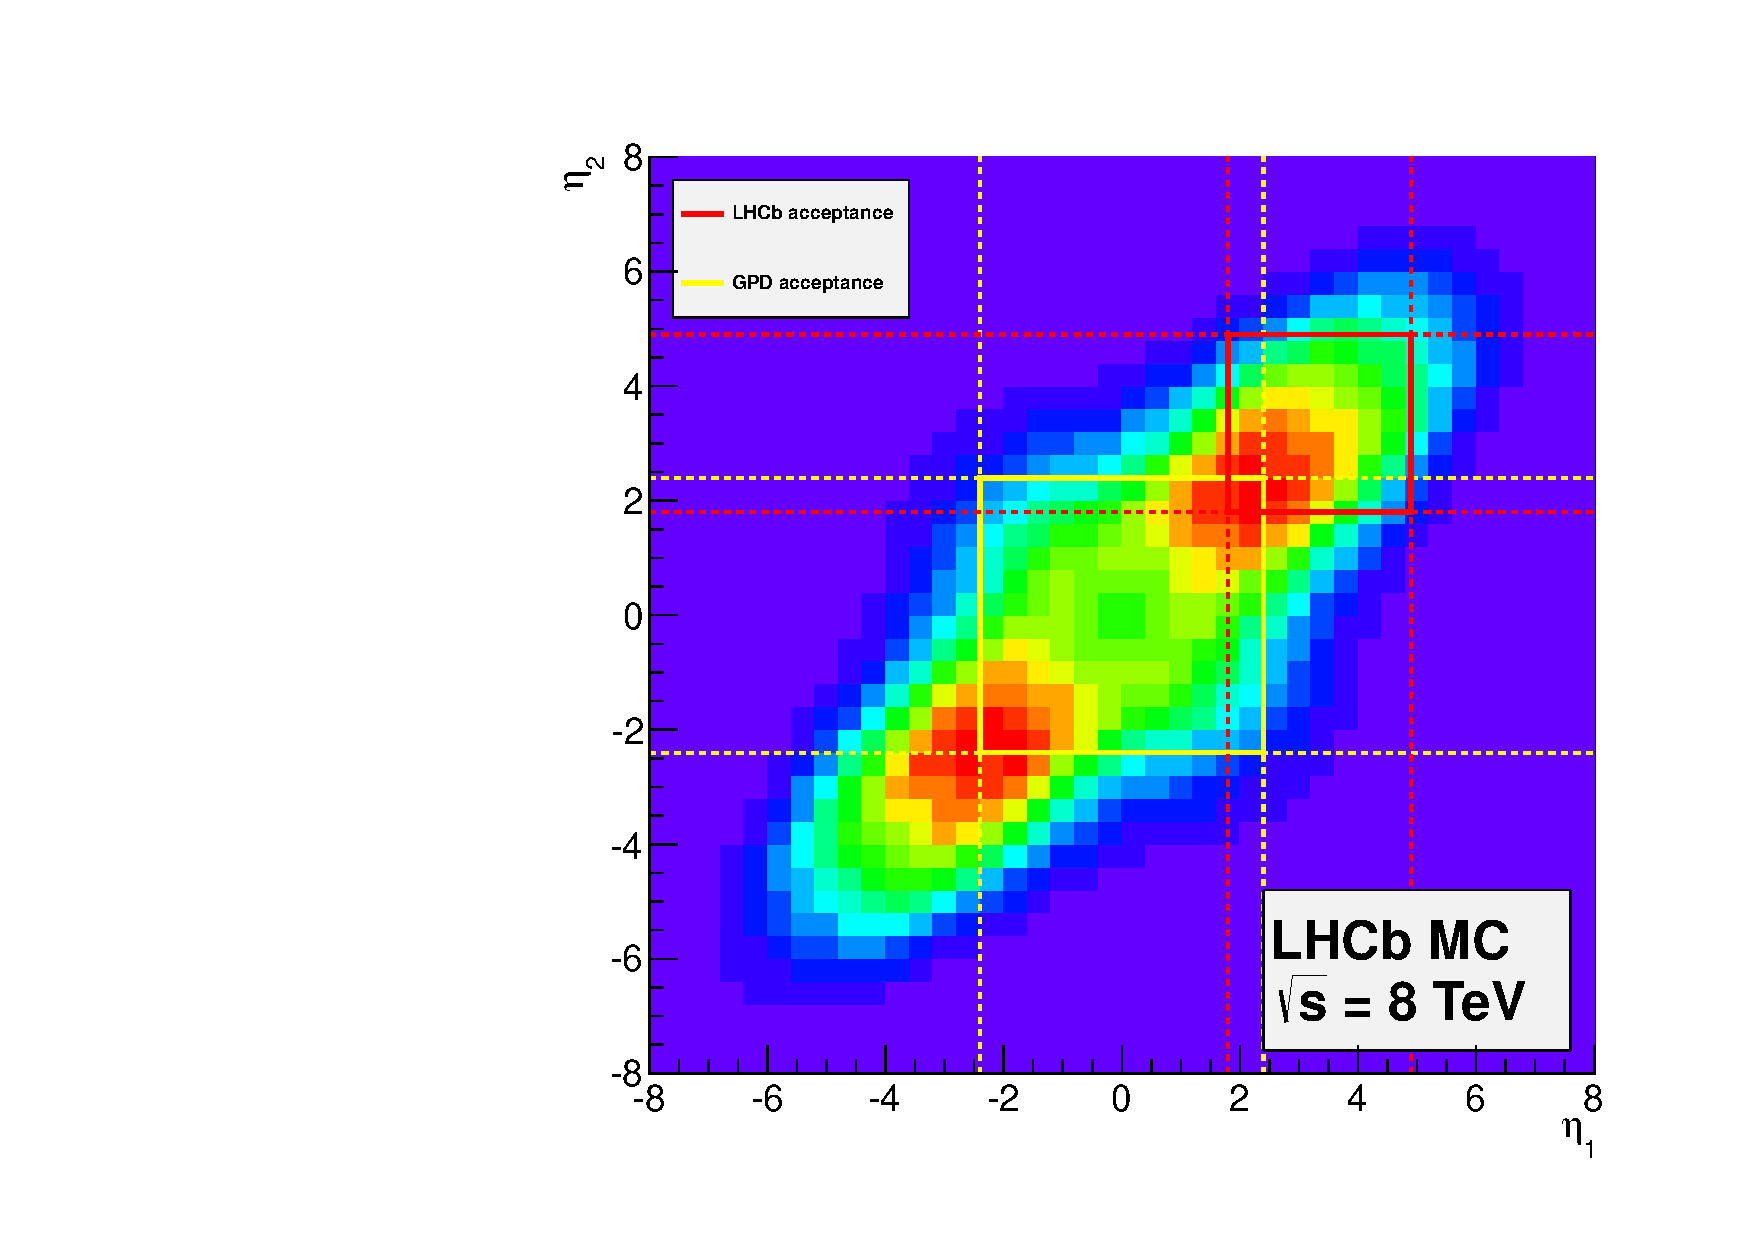
\includegraphics[scale = 0.4]{figs/detector/Acceptance.pdf}%
	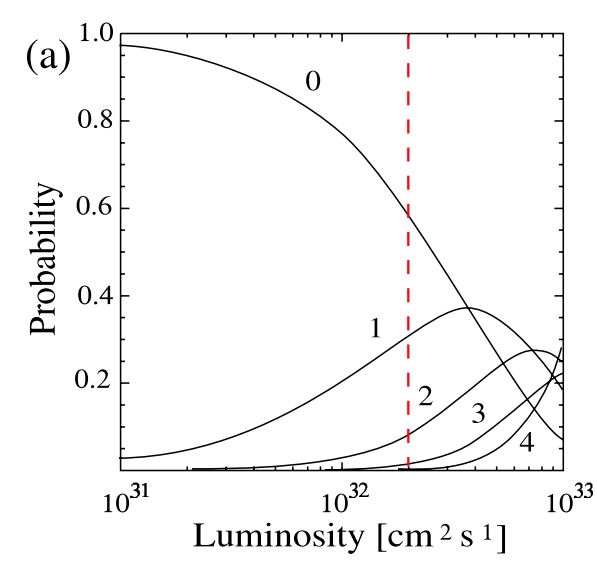
\includegraphics[scale = 0.5]{figs/detector/ProbInt.png}
	\caption{Angular production and acceptance of LHCb's $b\bar{b}$ pair (in red) as well as General Purpose Detector (in yellow). \Gls{LHCb} covers region with highest production cross-section at 8 \tev. These plots were produced using PYTHIA8 \cite{pythia8} simulation. This plot was taken from \cite{acceptance} (left). Probability of interaction per bunch crossing as a function of instanteneous luminosity. This figure was obtained from \cite{Raven:2007zi} (right).}
	\label{fig:Acceptance}
\end{figure}

The angular coverage of \Gls{LHCb} is formally defined using pseudorapidity $\eta$, 

\begin{equation}
	\eta = -\ln (\tan\frac{\theta}{2})
\end{equation}	
where $\theta$ is defined in~\autoref{fig:LHCbDetector}. \Gls{LHCb} detector, hence, covers the region $2<\eta<5$. The production cross-section of the fundamental process of $pp\rightarrow b\bar{b}X$ was measured in this region yielding, $\sigma (pp\rightarrow b\bar{b}X)$= 75.3$\pm$5.4$\pm$13.0 $\mub$b at 7 \tev \cite{LHCb-PAPER-2010-002} and 144$\pm$1$\pm$21 $\mub$ at 13 \tev \cite{LHCb-PAPER-2016-031}, which shows that the production cross-sections scales roughly linearly with the centre-of-mass energy. Assuming design conditions of LHCb, seen in~\autoref{tab:runcond}, 2$\fb^{-1}$ of data would correspond to $10^{12}$ of $b\bar{b}$ pairs being produced. 

\begin{figure}
	\centering
	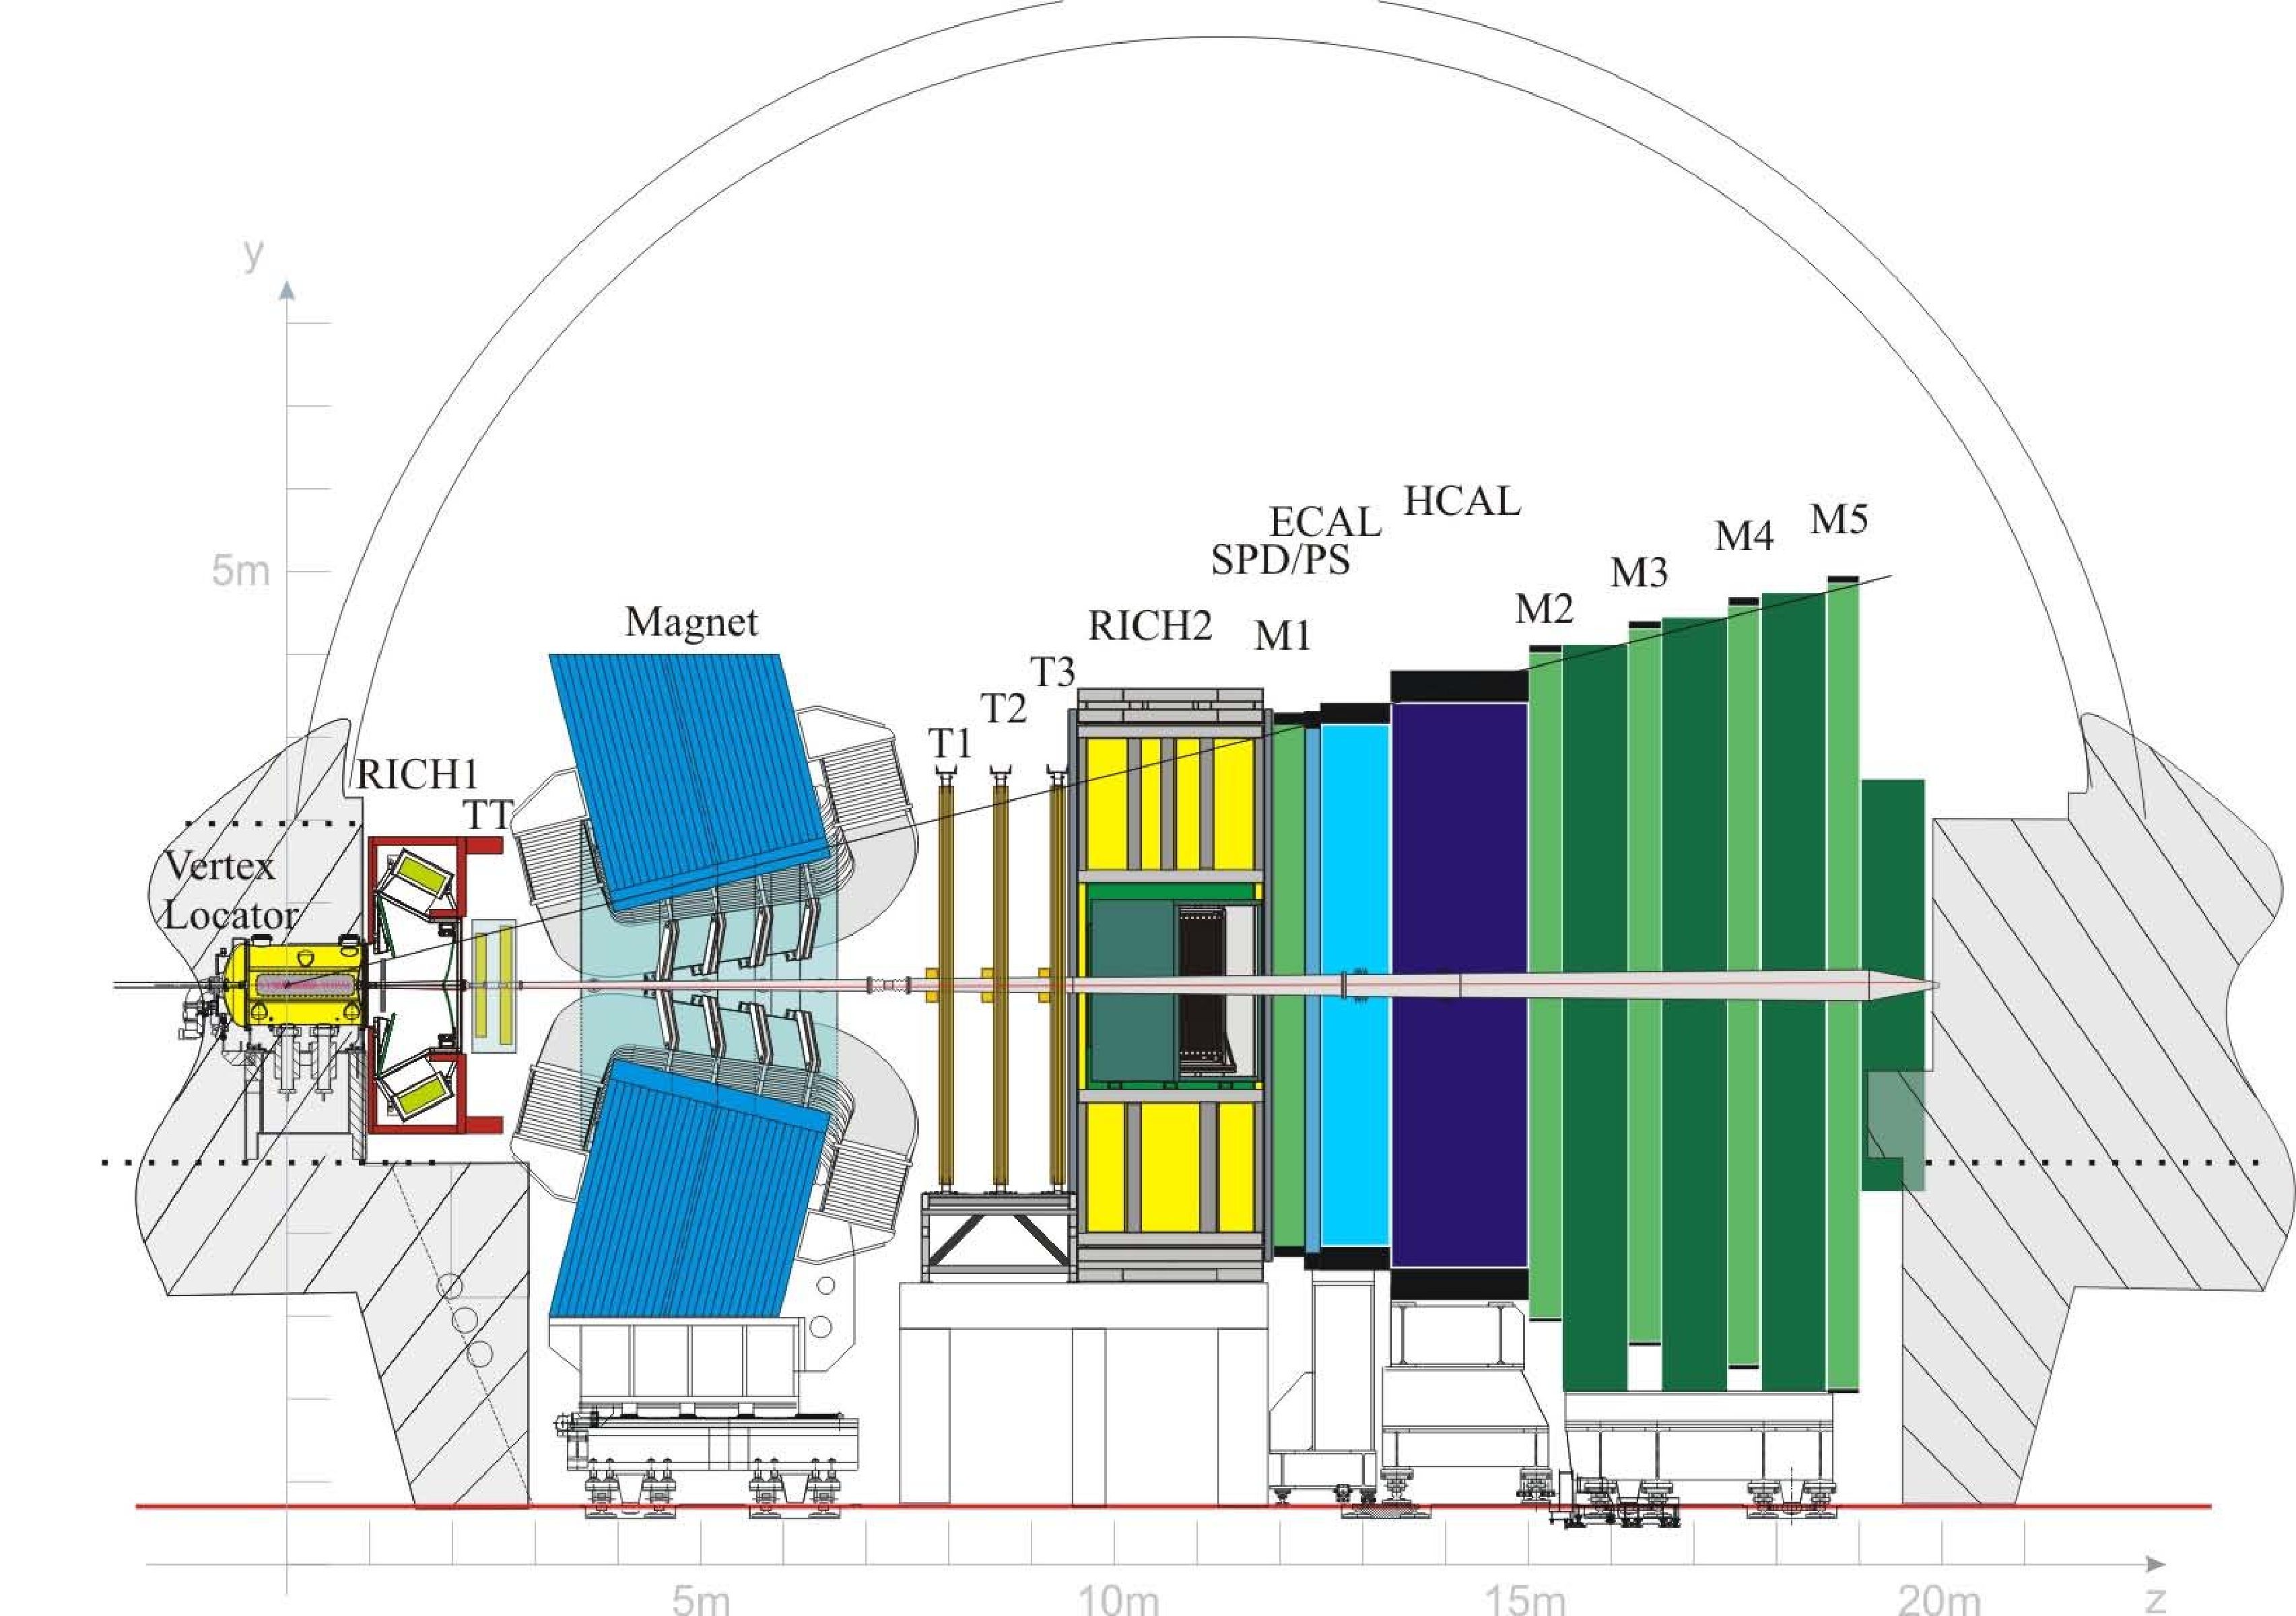
\includegraphics[scale = 0.15]{figs/detector/lhcbdet.pdf}
	\caption{The schematic slice of \Gls{LHCb} detector in $y,z$ plane where $z$ is defined to be the direction parallel to beamline, and $x,y$ define the plane perpendicular to the beamline. $\theta$, the opening angle in y-z plane with $\theta$ = 0 along $z-axis$. The figure was taken from \cite{LHCbdetector}.}
	\label{fig:LHCbDetector}
\end{figure}

Despite such impressive statistics of $b\bar{b}$ pairs available to \Gls{LHCb}, the bottleneck arises in much more copious inelastic background. It mostly originates from soft QCD processes which are related to the amount of pile-up, the visible number of $pp$ interaction in the visible events. By looking at the probability of number of $pp$ interaction per bunch crossing as a function of luminosity, shown in~\autoref{fig:Acceptance}, it can be noted that the maximum probability for only one $pp$ interaction (and hence minimizing the background) is found to be at $\sim 2 \times10^{32} cm^{-2} s^{-1}$, hence the LHCb design luminosity. In addition, to keep the occupancy of the detector reasonable, global event cuts, \textit{GEC}s, are put in the place, where only events with 600 (in 7,8 \tev) and 450 (in 13 \tev) tracks and less are allowed to be processed.

As \Gls{LHCb} requires much lower luminosity compared to other LHC detectors, it is achieved by LHCb-specific control of luminosity known as \textit{luminosity levelling}. This procedure achieves stable instantenous luminosity by controlling that the two beams do not collide straight head-on at collision point, but are moved with respect to each other. It limits the effects of luminosity decay, which can lead to trigger alterations during specific data taking run, resulting in systematic uncertainties.


So far, the detector has been running since 2010, with collected integrated luminosity shown in~\autoref{fig:lhcbintlumi}. As compared to \Gls{ATLAS} and \Gls{CMS} the integrated luminosity is much lower, due to allowed pile-up conditions. In 2017, there were two $pp$ collision energies at which the data was taken: at $\sqrt(s)$  = 13 and 5 TeV. Run \Rn{1} data-taking (2010-2012) was paused by Long Shutdown 1 (\Gls{LS1}) and followed with Run \Rn{2} data-taking (2015-2018). The summary of LHCb running conditions is provided in~\autoref{tab:runcond}, showing the evolution of the instantenous luminosity as well as the frequency of collisions compared to the design proposal.
%Formally \Gls{LHCb}   detector is placed along the beamline, where $x,y,z$ a spectrometer which cover the region of 300 \mrad defined a
%http://lhcb.web.cern.ch/lhcb/speakersbureau/excel/default.html

%\begin{figure}
%	\centering
%	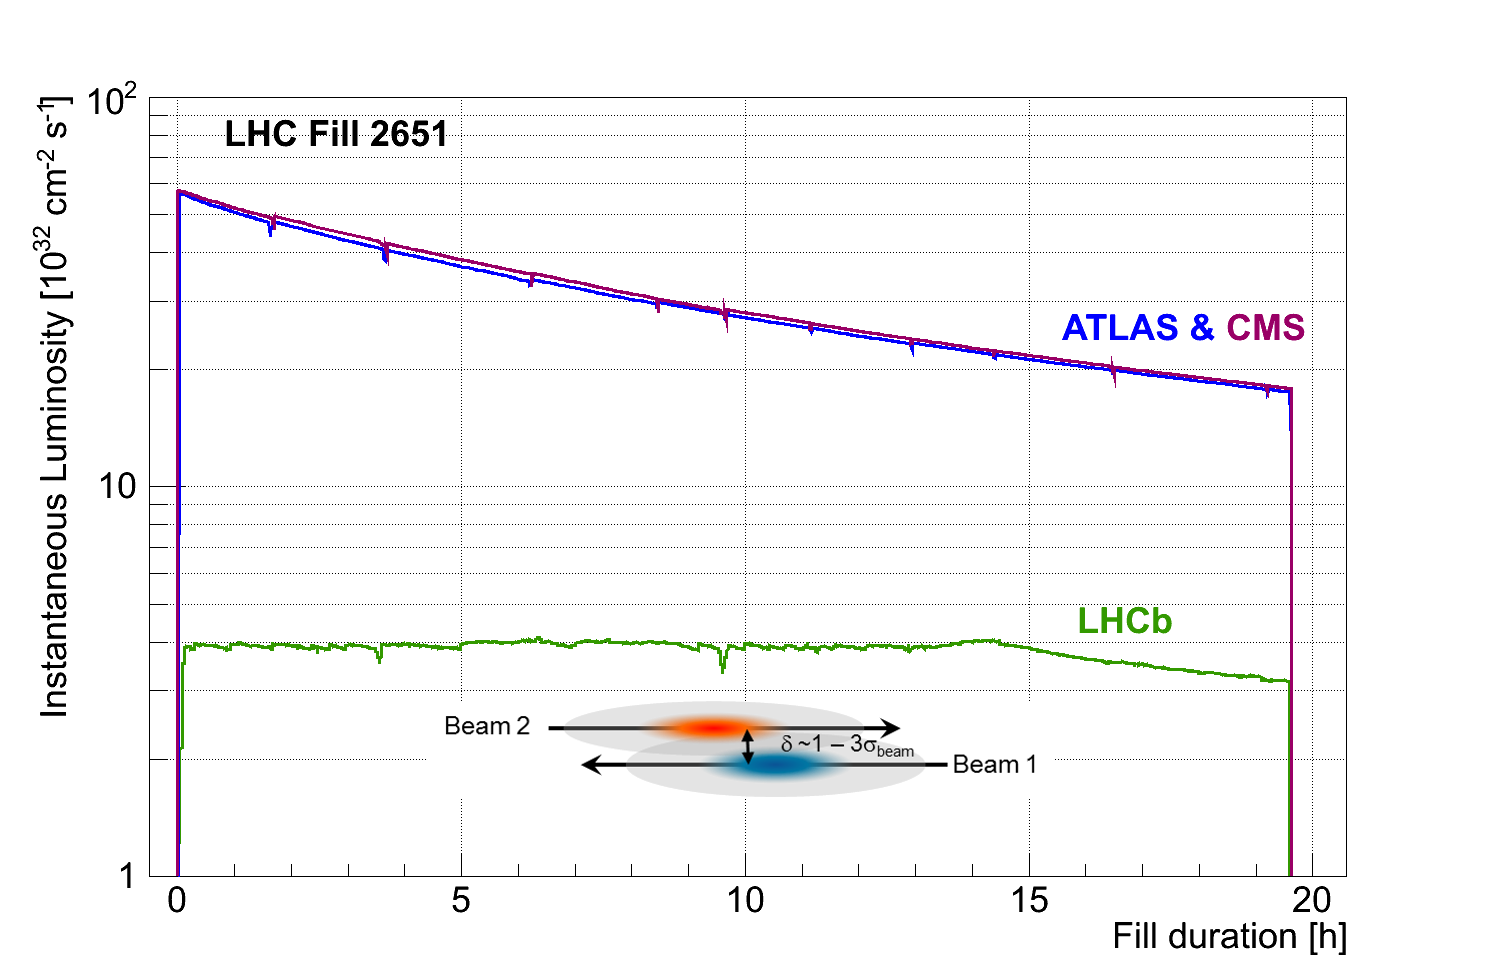
\includegraphics[scale = 0.5]{figs/detector/lumicompare.png}
%	\caption{Integrated luminosity collected in different years of data-taking. This plot is taken from \cite{lumiover}.}
%	\label{fig:lhcbintlumi}
%\end{figure}



\begin{table}[!h]
	\centering
	\hspace*{-0.8cm}
	\begin{tabular}{l c c }
		\hline
		year & $\sqrt(s)$ [TeV] & Instantenous Luminosity $\mathcal{L}$ [$\times10^{32} cm^{-2}	s^{-1}$] \\ \hline
		Design & Up to 14 & 2\\
		2011 & 7 & $\sim$ 3.0-3.5 \\
		2012 & 8 & $\sim$ 4.0 \\
		2015 & 13 & $\sim$ 0.5-4.5 \\      
		2016 & 13 & $\sim$ 4.0  \\      
		2017 & 13 & $\sim$4.0-6.0 \\\hline      
	\end{tabular}
	\caption{Running conditions of LHC and \Gls{LHCb} in different years of data-taking. The statistics of LHCb's instantenous luminosity is extracted using run database. }
	\label{tab:runcond}
\end{table}   

\begin{figure}
	\centering
	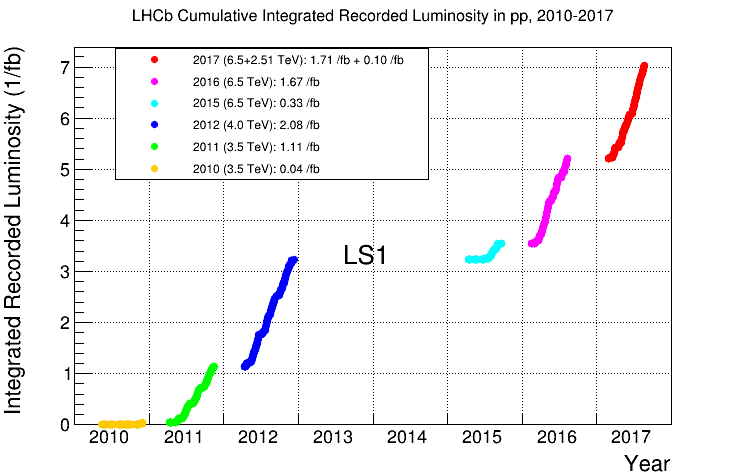
\includegraphics[width = 0.5\textwidth]{figs/detector/intlumi.png}%
        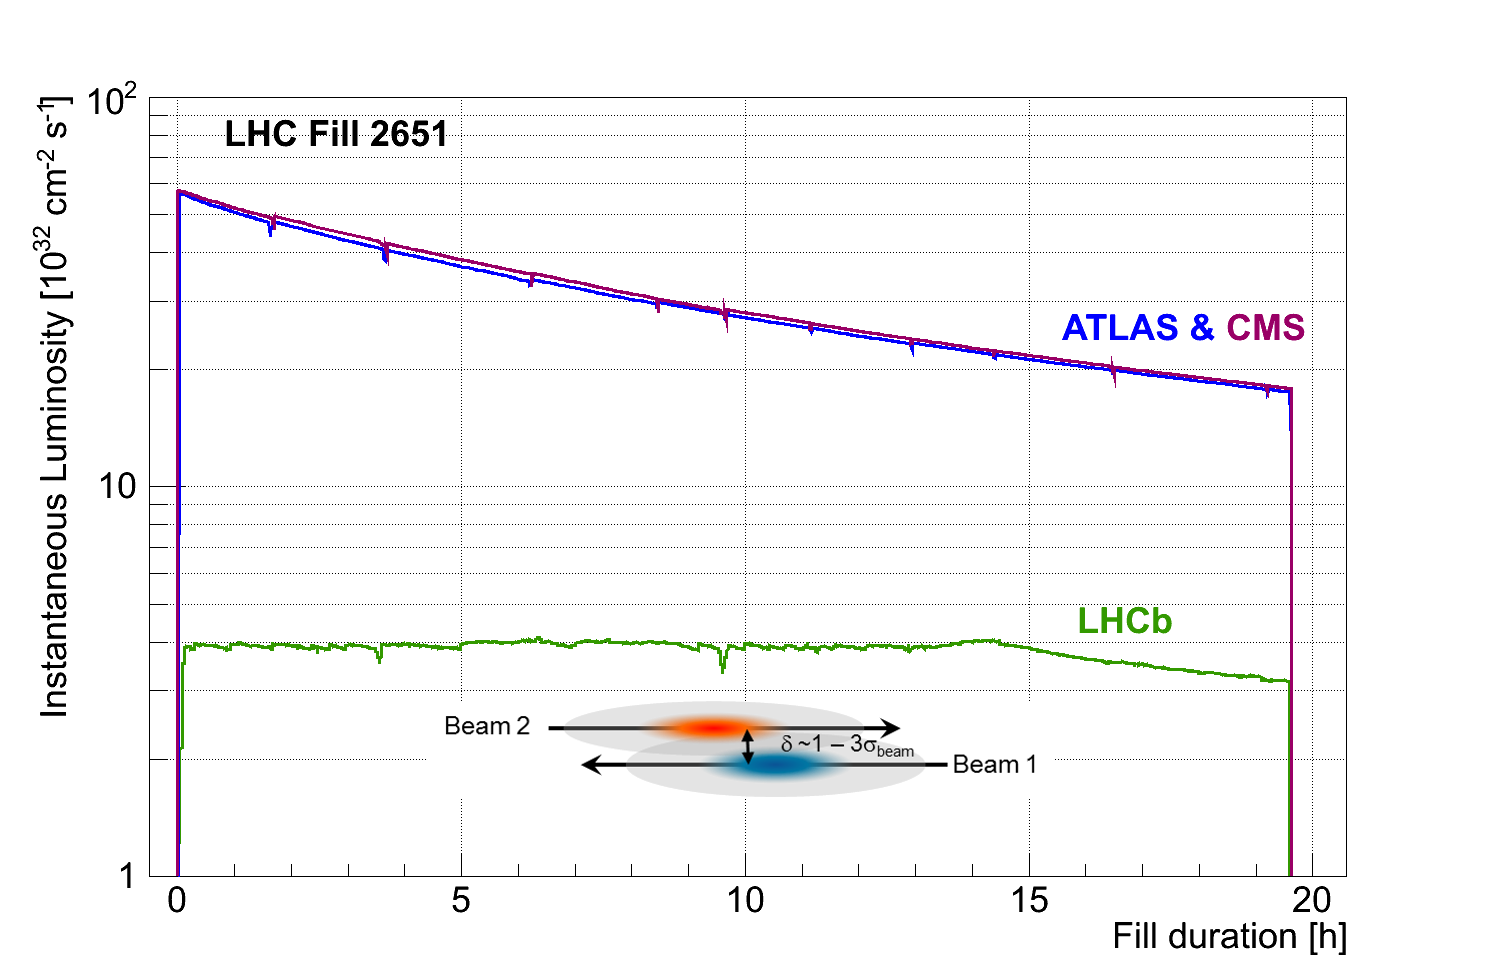
\includegraphics[width = 0.5\textwidth]{figs/detector/lumicompare.png}
	\caption{Integrated luminosity collected in different years of data-taking. This plot is taken from \cite{lumiover} (left). Development of the instantaneous luminosity for \Gls{ATLAS}, \Gls{CMS} and \Gls{LHCb} during LHC fill 2651. After ramping to the desired value of $4\times10^{32}cm^{-2}s^{-1}$
for LHCb, the luminosity is kept stable in a range of 5$\%$ for about 15 hours by adjusting the transversal beam overlap. The difference in luminosity towards the end of the fill between ATLAS, \Gls{CMS} and \Gls{LHCb} is due to the difference in the final focusing at the collision points, commonly referred to as the beta function, $\beta^{*}$. This plot was obtained from \cite{LHCb-DP-2014-002} (right).}
	\label{fig:lhcbintlumi}
\end{figure}

In the following sections, brief discussion of different subdetectors is presented. Both hardware and software overview will be presented with particular emphasis given to Muon Station and Simulation of LHCb.

\section{VErtex LOcator}
The closest detector around the collision point is VErtex LOcator (\Gls{VELO}). This silicon-strip based detector, that extends 1 \m along the beam axis, is primarily used for to distinguish events from promt background. The typical differing property of a $B$ hadron decay includes large impact parameter (\Gls{IP}), the minimal distance between the track and primary vertex, in addition to significantly higher transverse momentum $p_{T}$. Main uses of this subdetector include finding: 
\begin{itemize}
\item primary vertices positions
\item secondary vertices of short-lived particles (heavy quark hadrons)
\item tracks that did NOT originate from primary vertex
\end{itemize}.


\begin{figure}[!h]
	\centering
	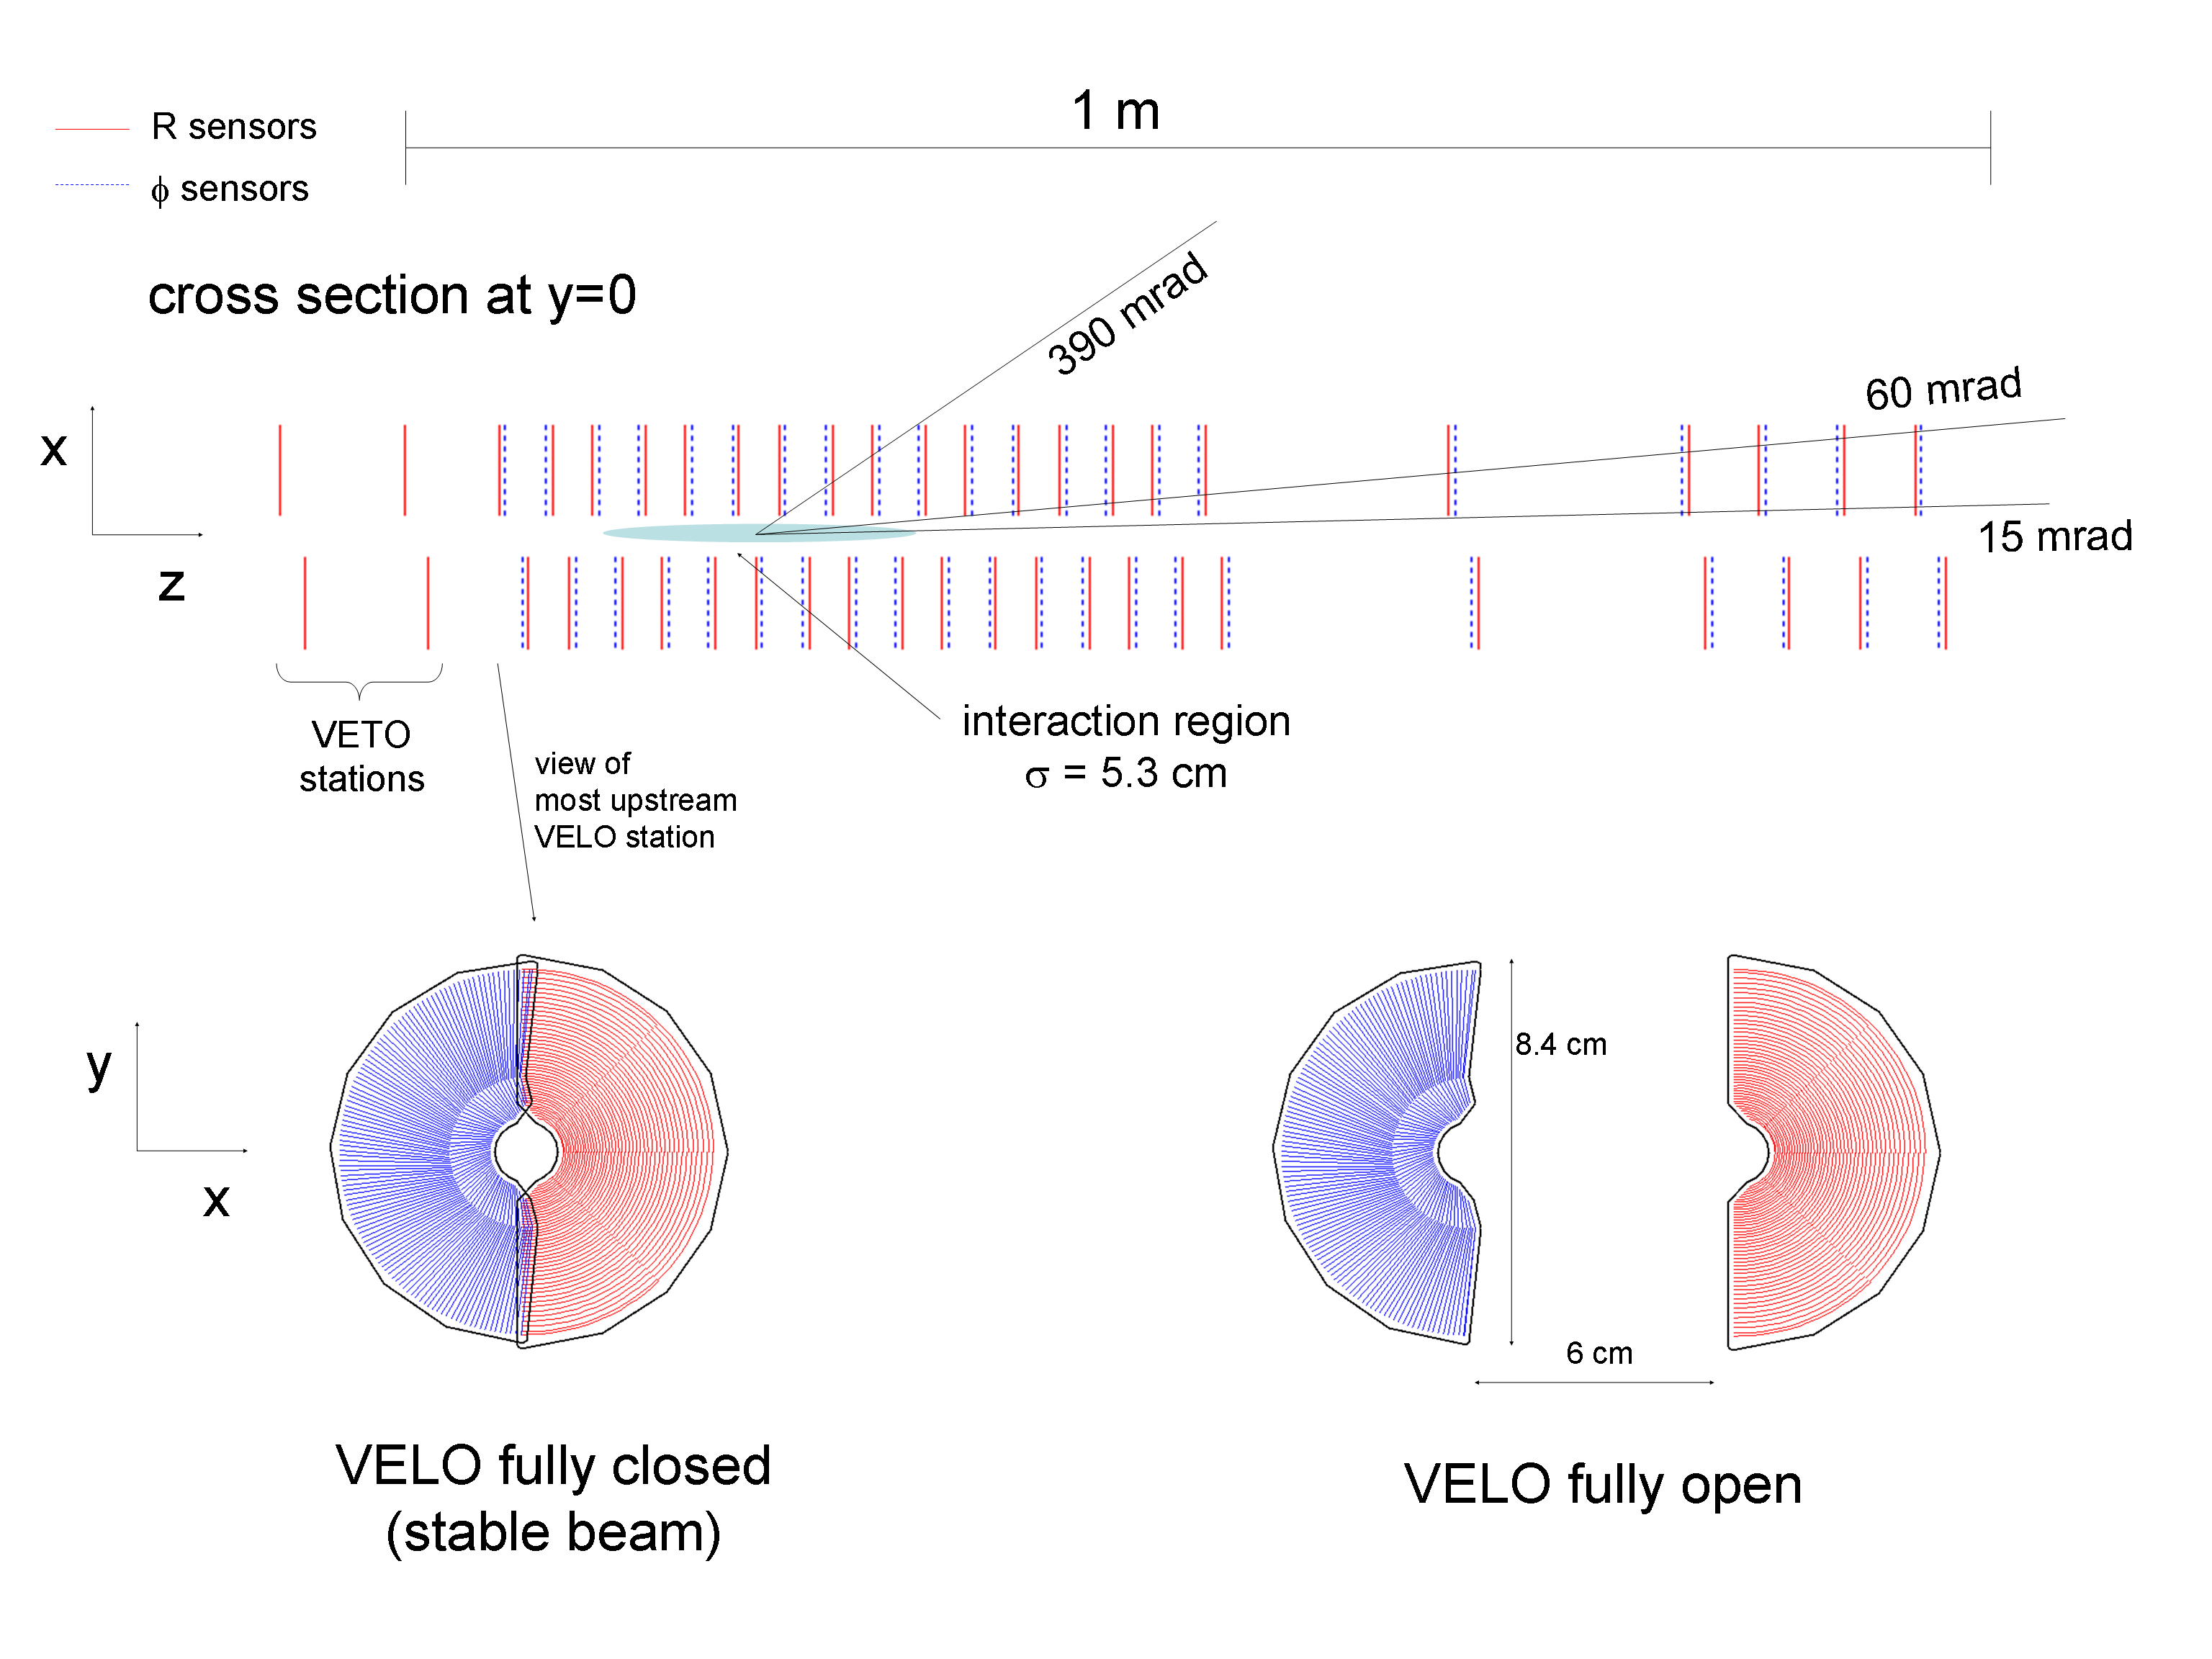
\includegraphics[width = 0.75\textwidth]{figs/detector/veloOverview.png}
        %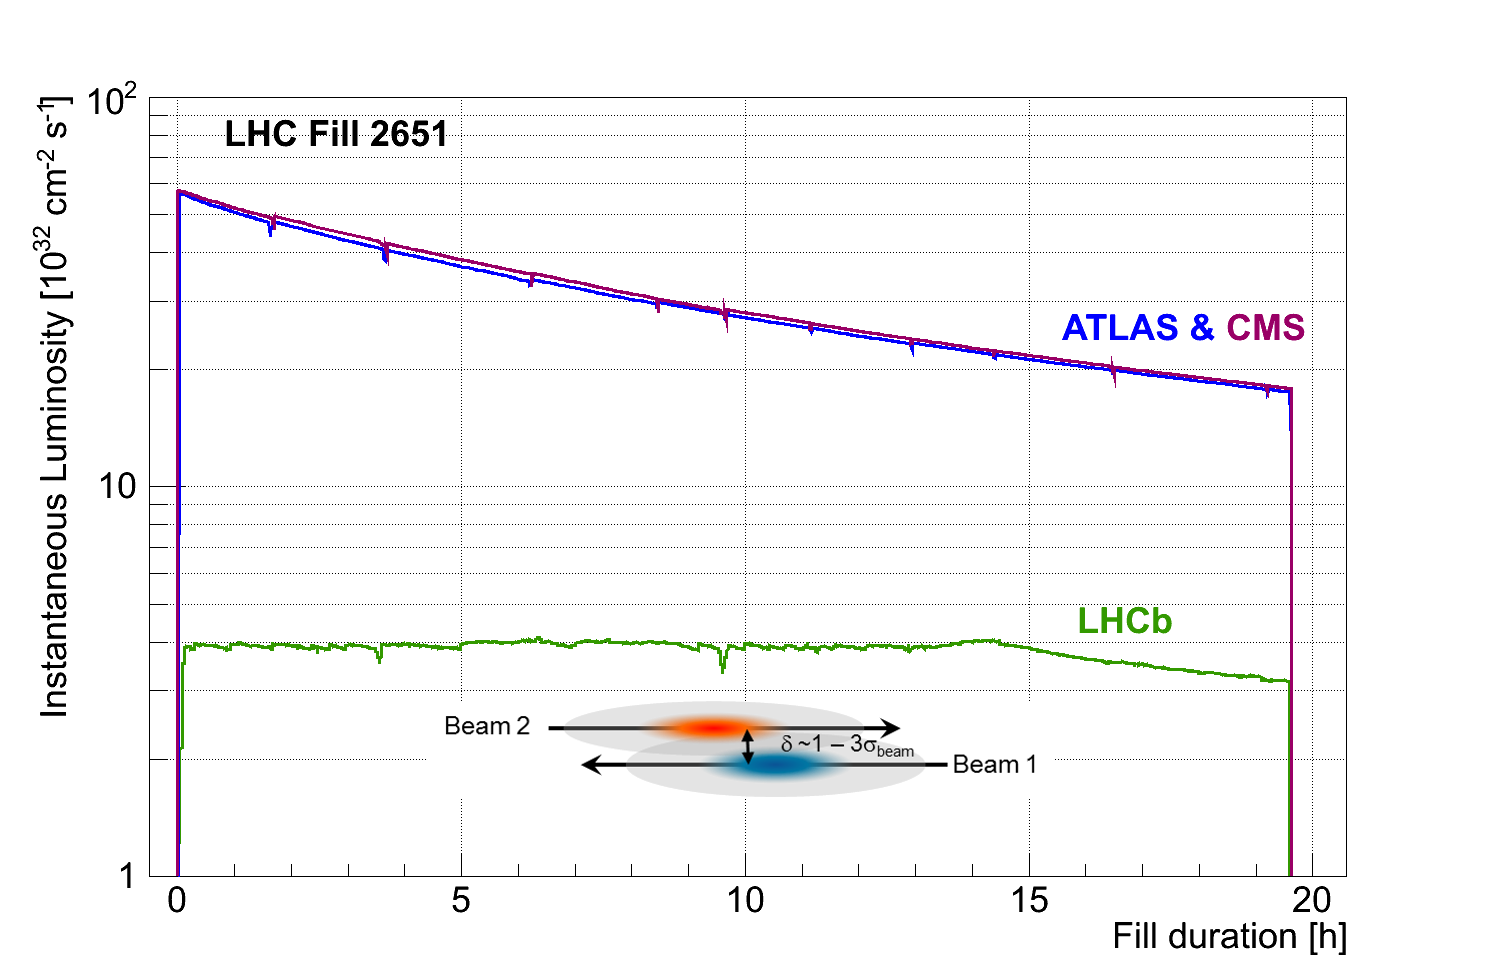
\includegraphics[width = 0.5\textwidth]{figs/detector/lumicompare.png}
	\caption{ Schematic plot of \Gls{VELO} detector configuration along the beam pipe showing the layout as well as positions while in stable beams (discs have slight overlap) and injection. Figure taken from \cite{det_paper}.}
	\label{fig:veloover}
\end{figure}

The detector consists of two sets of 21 silicon modules positioned around the beam pipe, where each module has 2 types of half-moon-shaped discs as seen in~\autoref{fig:veloover}. In the first disc type the strips are arranged to provide radial information ($R$), whereas the second type provides azimuthal ($\phi$) information. As $pp$ interaction point brings high radiation dose for this detector, the first sensitive strip starts only at a distance of 8 \mm once stable beams are declared. Throughout the beam injection, when the beam radius may be larger, the two sets are moved away 3 \cm perpendicularly from the interaction point. For the ($R$) sensor, the individual module's strip pitch, distance between two strips, varies from 38 $\mum$ to 102 $\mum$ away from the beam pipe, so that the hit occupancy is roughly even. Each \Gls{VELO} half is kept within an alluminum welded box causing material overlap once stable beams are declared. These boxes then create their own vacuum which is different to the nominal LHC vacuum in order to protect the detector from any elelctromagnetic interference with the beam. 

This setup brings outstanding hit resolution (4-40$\mum$), which in turn allows for very high impact parameter resolution and very good primary vertex resolution, as seen in~\autoref{fig:veloIPres}. This is indispensable not only in order to perform the precise measurements of $B$ and $D$ lifetimes, but also to resolve oscillations caused by $B^{0}_{s}-\bar{B}^{0}_{s}$ mixing occuring at 3 trillion \hz rate.

\begin{figure}[!h]
	\centering
	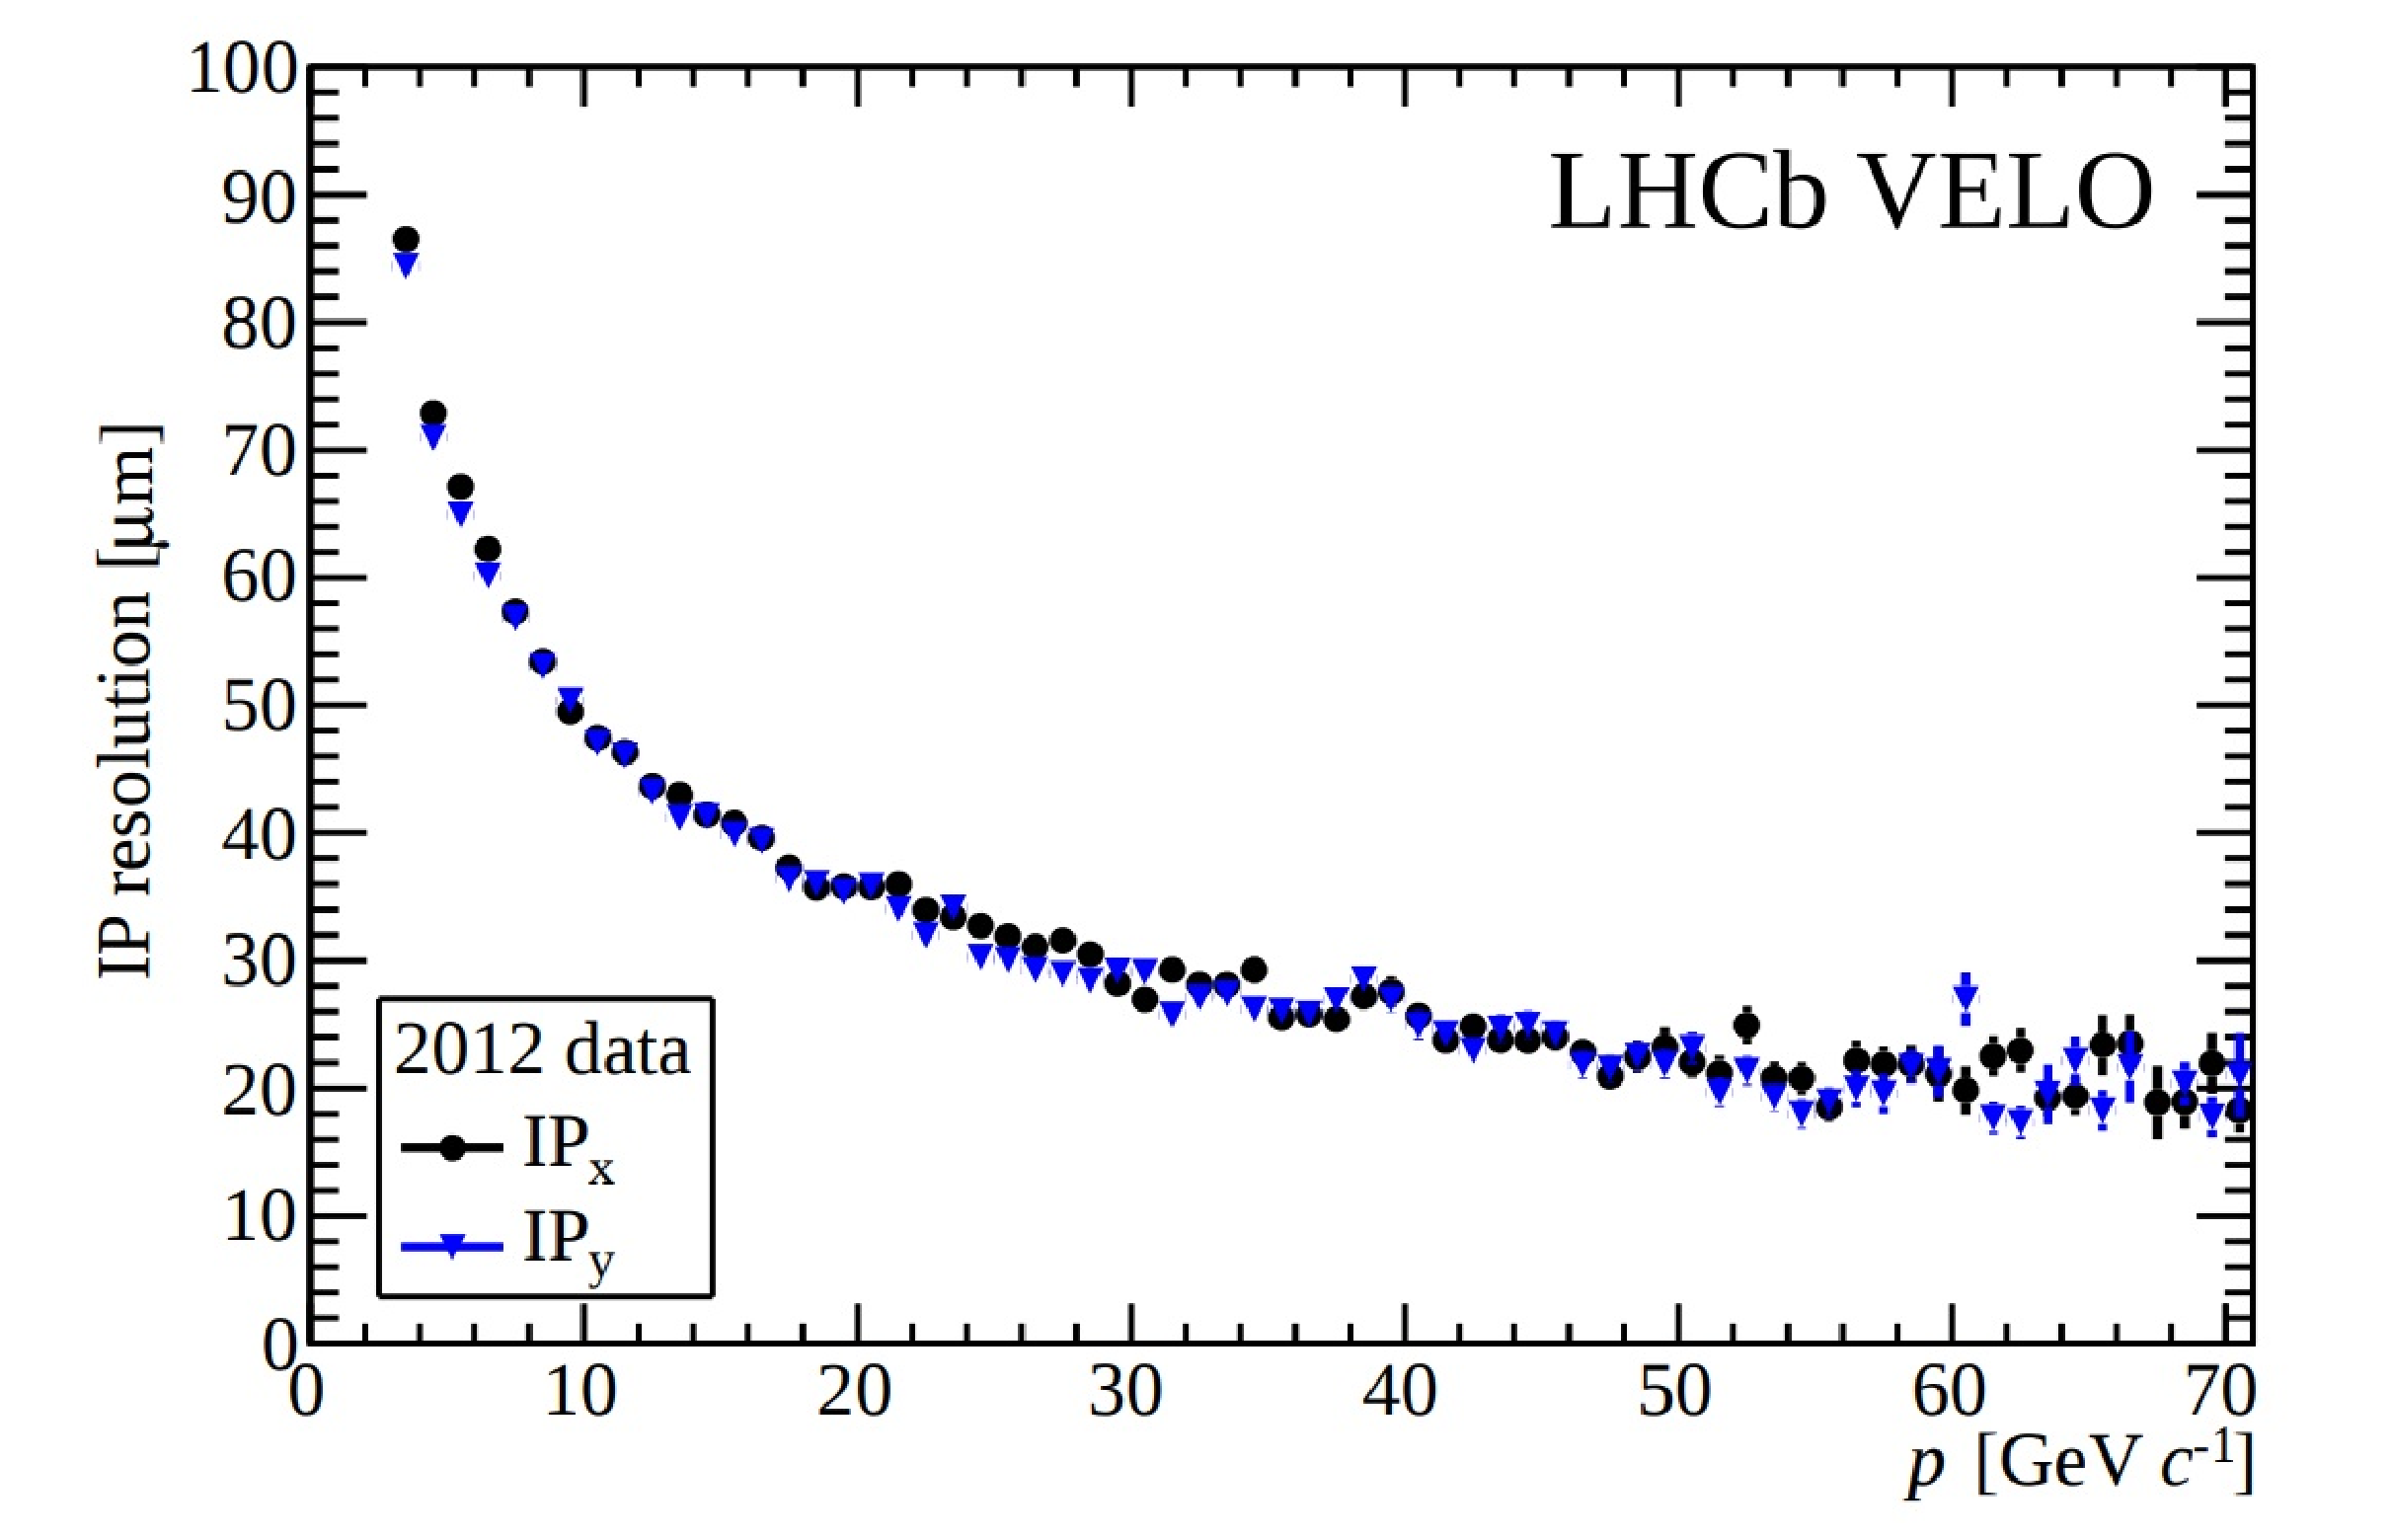
\includegraphics[width = 0.5\textwidth]{figs/detector/IPresmhm.eps}%
        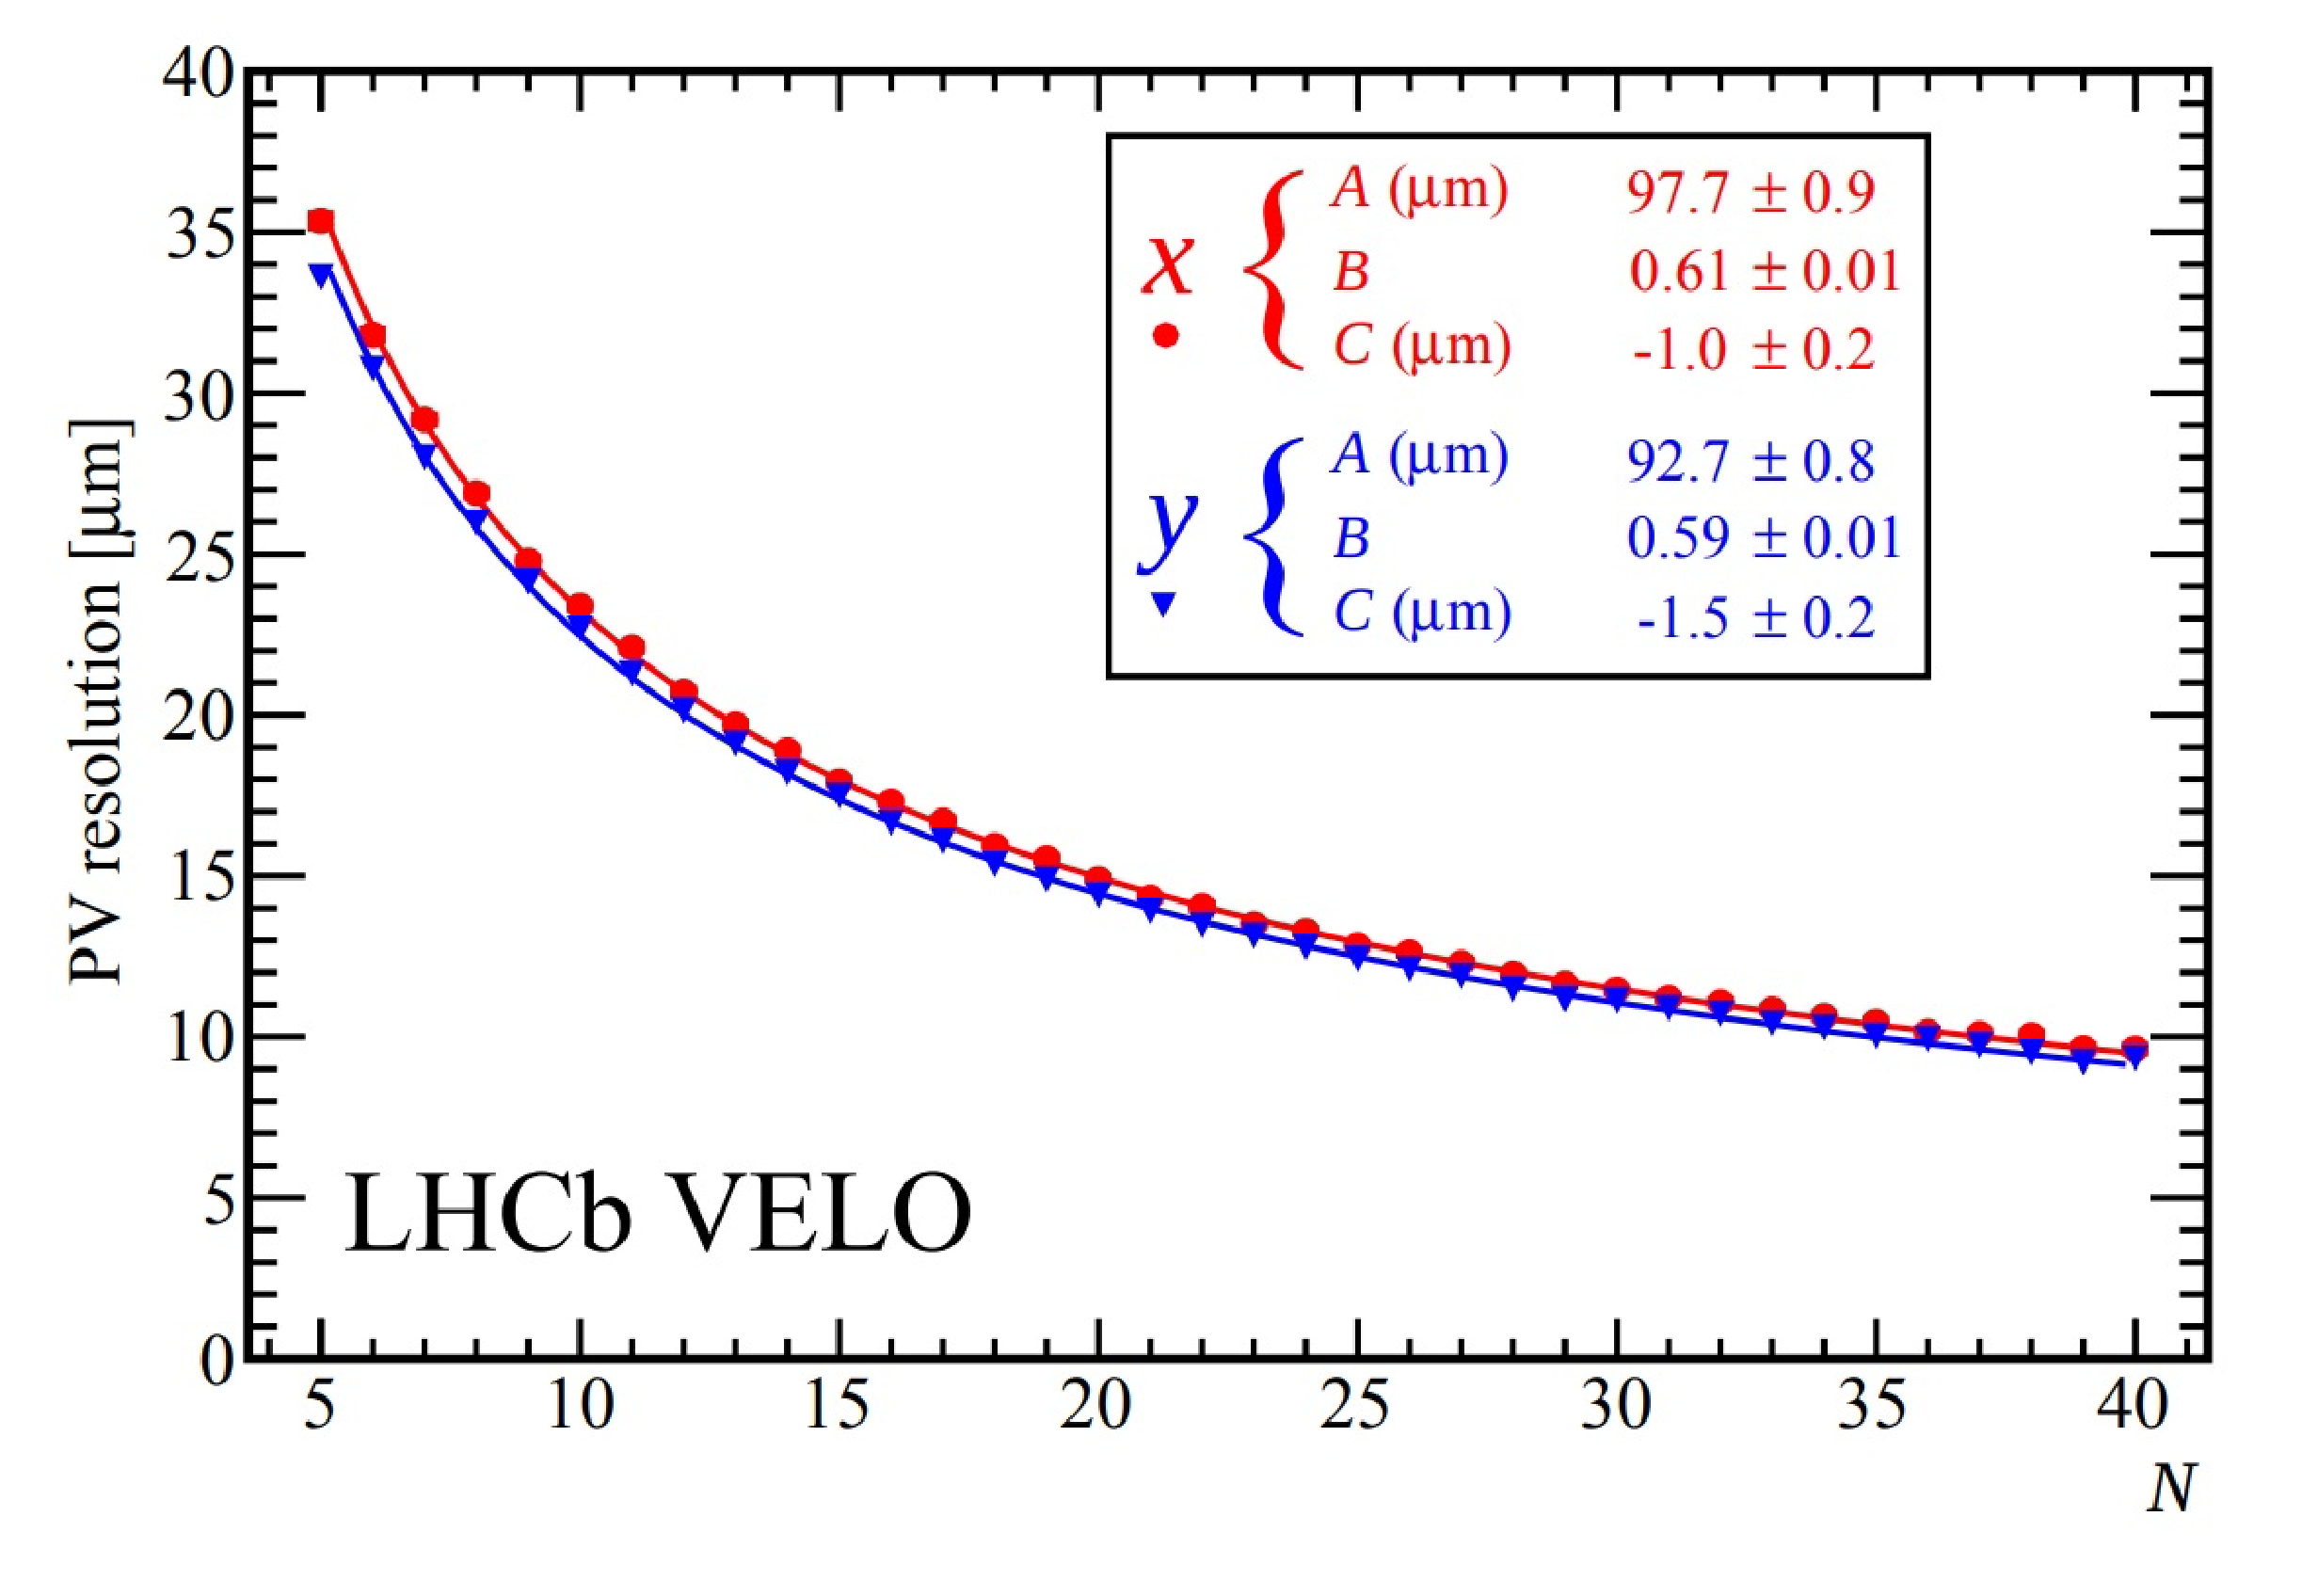
\includegraphics[width = 0.5\textwidth]{figs/detector/PVres.eps}
	\caption{Two key variables which quantify performance of the \Gls{VELO} detector. \Gls{IP} resolution which is worse for low momentum tracks (left) and \Gls{PV} resolution dependent on the number of tracks forming the primary vertex $N$ (right). Figures taken from \cite{LHCbVELOGroup:2014uea}.}
	\label{fig:veloIPres}
\end{figure}


\section{Tracking System}
In addition to tracking information provided by \Gls{VELO}, the trajectories of charged particles are monitored by series of tracking subdetectors. The main task of these tracking subdetectors is to provide efficient reconstruction and precise measurement of particle's momentum. There are four tracking stations apart from \Gls{VELO}: Tracker Turicensis (\Gls{TT}), positioned upstream from magnet, and  \Gls{Tstation} tracking stations on the other side from the magnet. The 10 \m dipole magnet with $\approx$ 4 Tm integrated field provides enough strenght to bend charged particles with $p$ of 200 $GeV/c^{2}$.      

 Two different dectection technologies are used in these trackers reflecting the nature of track occupancy as function of distance from beam pipe. The tracker's part close to the beam pipe, \Gls{TT} station together with central region of T1-T3, also known as Inner Tracker (\Gls{IT}), expects higher occupancy and makes use of the the silicon microstrip detection mechanism. The outer part of \Gls{Tstation} stations, also known as Outer Tracker \Gls{OT}, is made of a straw-tube detectors. It measures the hit position by measuring the drift-time of ionized electrons. This two technologies are seen in~\autoref{fig:tracktype}. 

\subsection{Tracking Algorithms}
Different particles will leave different footprint in the detector. Charged particles will form tracks. Depending on presence of hits in individual subdetectors, they are grouped into several categories, visualized in~\autoref{fig:tracktype}.

\begin{figure}[!h]
	\centering
	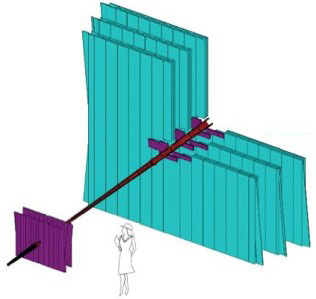
\includegraphics[width = 0.35\textwidth]{figs/detector/trackingsystem.jpg}%
	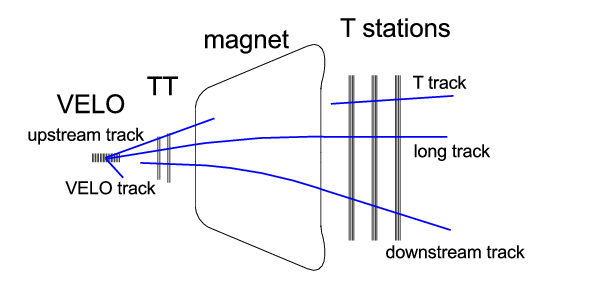
\includegraphics[width = 0.6\textwidth]{figs/detector/tracktype.png}
	\caption{ Visualisation of use of different technology with silicon technology in violet and straw-tube technology in cyan. The Figure was obtained in \cite{OT}(left). Track types visualisation depending on which track stations provided hits. For the study of \Bmumumu decays only, \Gls{longtrack}, are considered as muons will travel to the end of the detector leaving the hits all along. Figure is taken from \cite{LHCb-DP-2013-002} (right).}
	\label{fig:tracktype}
\end{figure}

%http://iopscience.iop.org/article/10.1088/1748-0221/3/08/S08005/pdf
%https://twiki.cern.ch/twiki/bin/view/LHCb/TrackingEffAbsLength /secondary interactions - hadronic int.

Most of the physics analyses use long tracks, tracks leaving hits in \Gls{VELO} and \Gls{Tstation}, as they give most precise momenta estimates.
VELO tracks leave hits only in $R$ and $\Phi$ sensor, but not in any other tracking stations, meaning that they must have left \Gls{LHCb} acceptance or they come from particles produced backwards and hence are useful for $PV$ reconstruction. Upstream tracks are formed by tracks leaving hits in \Gls{VELO} and TT only. These are usually low momentum particles, which are bent out \Gls{LHCb} acceptance while traversing the magnet. Long-lived particles such as $\Lambda$ or $K^{0}_{s}$ will only decay ouside of the \Gls{VELO} acceptance and hence will produce no hits until \Gls{TT} and \Gls{Tstation} forming downstream tracks. T-track is track type that only have hits in \Gls{Tstation}. Again this could be due to presence of long-lived particles or due to secondary interactions in the detector.   

In general, the track reconstruction software starts with \textit{pattern recognition}, where several hits in one part of a tracking subdetector are identified and form \textit{track seeds}, which are then extrapolated and combined with hits in other tracking subdetector provided this subdetector sits in low magnetic field. The long track candidates are formed and fitted with a Kalman filter\cite{Hierk:684697}, where because of the material present in the detector, corrections for energy losses as well as multiple scaterring are incorporated.

Sometimes \textit{pattern recognition} may combine random hits into a track, \textit{ghost track}, or several tracks could be made out of same hits, \textit{clone track}. Presence of these tracks are heavily suppresed with different techniques - such as establishing ghost probability - variable based on the output of neural network combining track $\chi^{2}$ and missing hits in the subdetectors.

Mass uncertainty is one of the crucial parameters to minimize as it provides opportunity for high precision measurements by better separations from backgrounds. It strongly correlates with momentum resolution that is obtained using tracking. Resulting relative momentum uncertainty (0.5-1.1\%) on long tracks using $J/\psi \rightarrow \mu^{+} \mu^{-}$ using \textit{tag and probe} can be seen in~\autoref{fig:momres}. It varies logarithmically with increasing momentum.


\begin{figure}[!h]
	\centering
	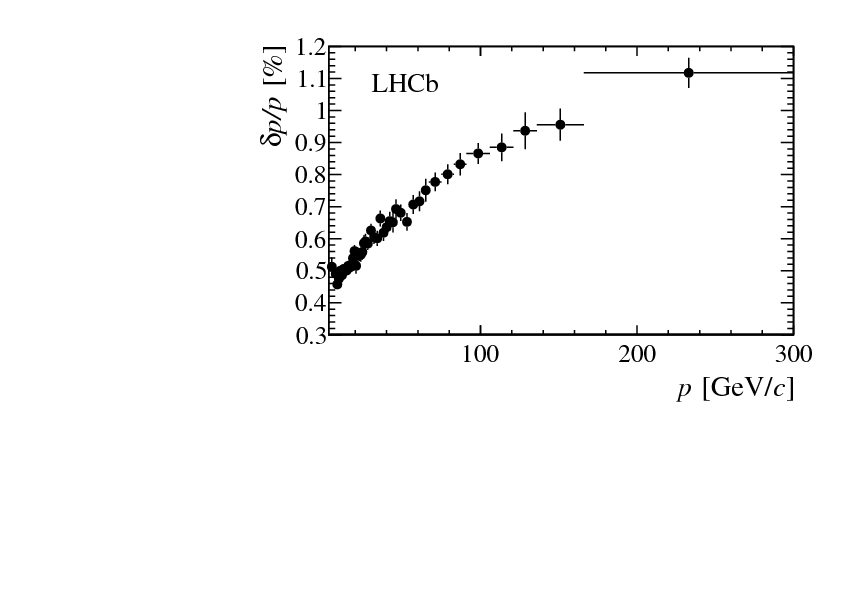
\includegraphics[width = 0.6\textwidth]{figs/detector/momresolution.png}
	\caption{Momentum resolution of long tracks measured using "tag and probe" method at LHCb. The decay channel $J/\psi^{+} \rightarrow \mu^{+} \mu^{-}$ is analyzed.}
	\label{fig:momres}
\end{figure}

\section{Ring Imaging Detectors}
Particle identification, \Gls{PID}, at \Gls{LHCb} relies heavily on two dedicated Ring Imaging subdetectors. These detectors take advantage of the phenomena, emission of Cerenkov light, which happens when a charged particle travels through a medium at a speed faster than the phase velocity of light in that medium. This cone of light is emitted at an angle $\theta$ with respect to the charged particle's trajectory. Using the knowlegde of refractive index of the medium, $n$, and momentum $p$ that is measured using tracking, mass $m$ of the particle can be obtained through:

\begin{equation}
	\cos\theta_{c} =  \frac{\sqrt{m^{2} + p^{2}}}{pn}.
\end{equation}

As the momentum and mass are intrinsic properties of passing particle, the momentum identification range is limited by the choice of medium, also known as radiator. For very low-momentum particle, as $\cos\theta_{c} \rightarrow 1$, the particle is not producing any Cerenkov light cone. At the very high momentum, as $\cos\theta_{c} \rightarrow 0$, there is saturation point as all species of particles will emit the light at the same Cherenkov angle, hence all the discriminating power will be lost.

Low momentum (2-60 \gev) particles are identified in the upstream RICH1 detector and high momentum particles (15-100) \gev are analyzed downstream in RICH2. RICH1 covers $\pm$ 25-300 mrad in x-z plane, $\pm$ 250 mrad in the x-y plane, using either gaseous Aerogel ($n=1.03$) and $C_{4}F_{10}$ ($n = 1.0014$) as radiators. RICH2 has more limited acceptance of $\pm$15-120 mrad in x-y plane and $\pm$100 mrad in x-z plane and uses $CF_{4}$ as radiator, with lower $n=1.0005$. The discrimination power between different particles can be seen~\autoref{fig:richres}. 


Both RICH1 and RICH2 use set of spherical primary mirrors to guide the photons onto the flat secondary mirrors which are then further focused into Cerenkov rings onto the surface of Hybrid Photon Multipliers, \Gls{HPD}. The schmematic view of a particle passing through RICH1 can be also be seen in~\autoref{fig:richres}. 


\begin{figure}[!h]
	\centering
	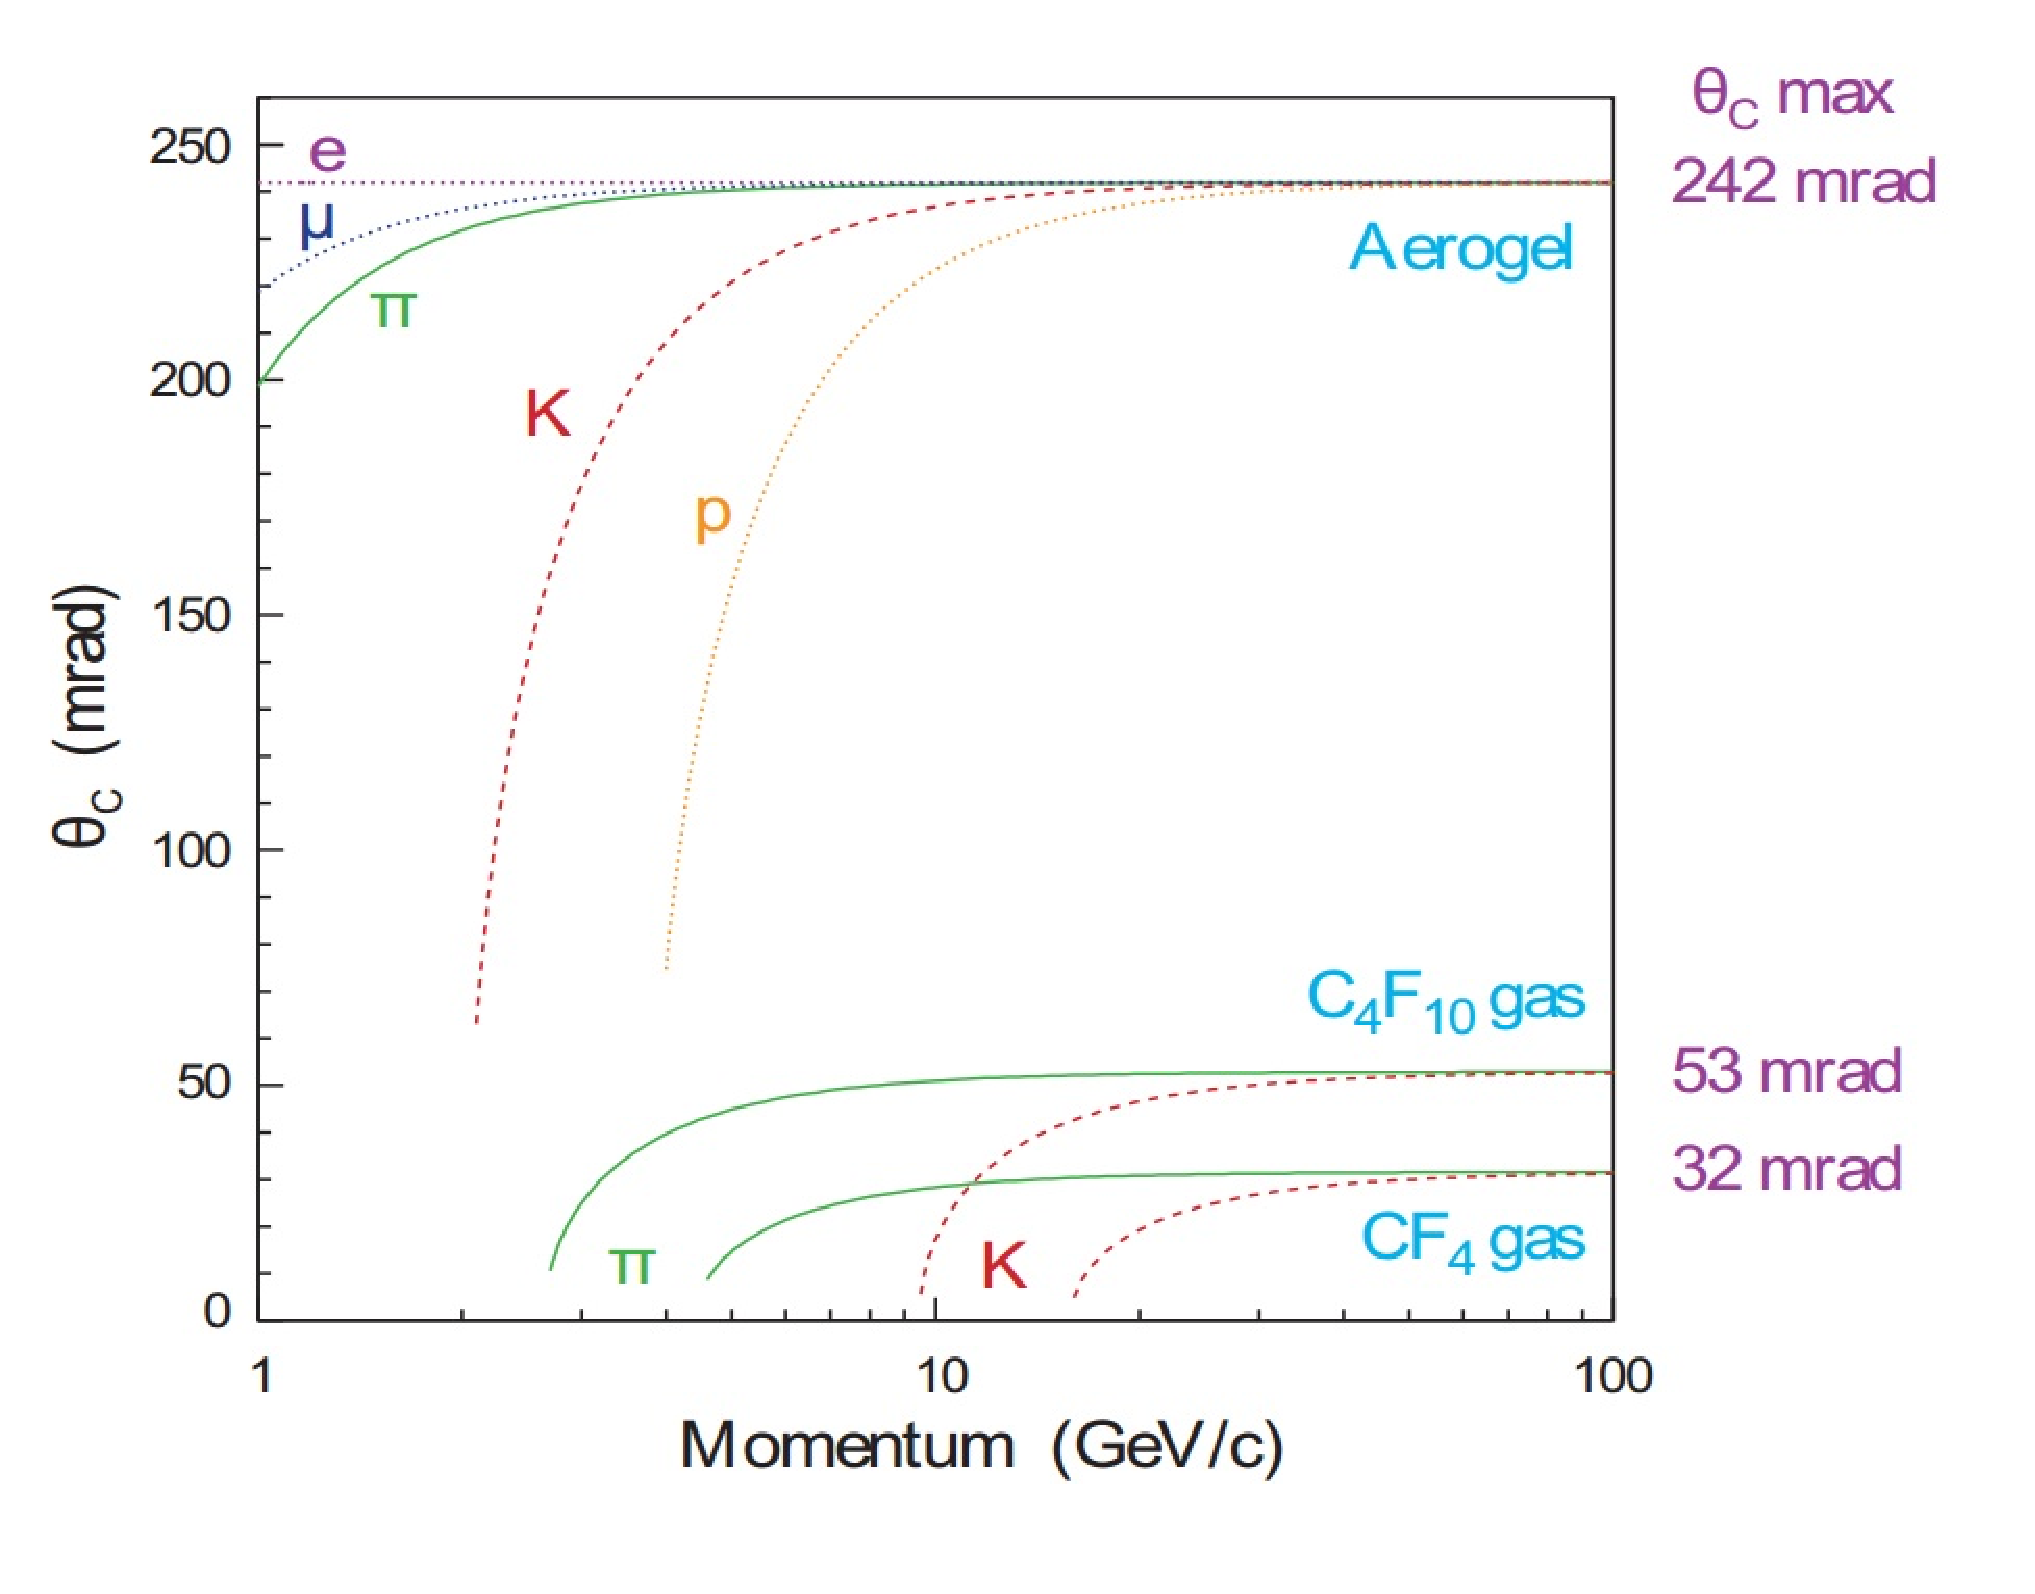
\includegraphics[width = 0.55\textwidth]{figs/detector/richres1.eps}%
	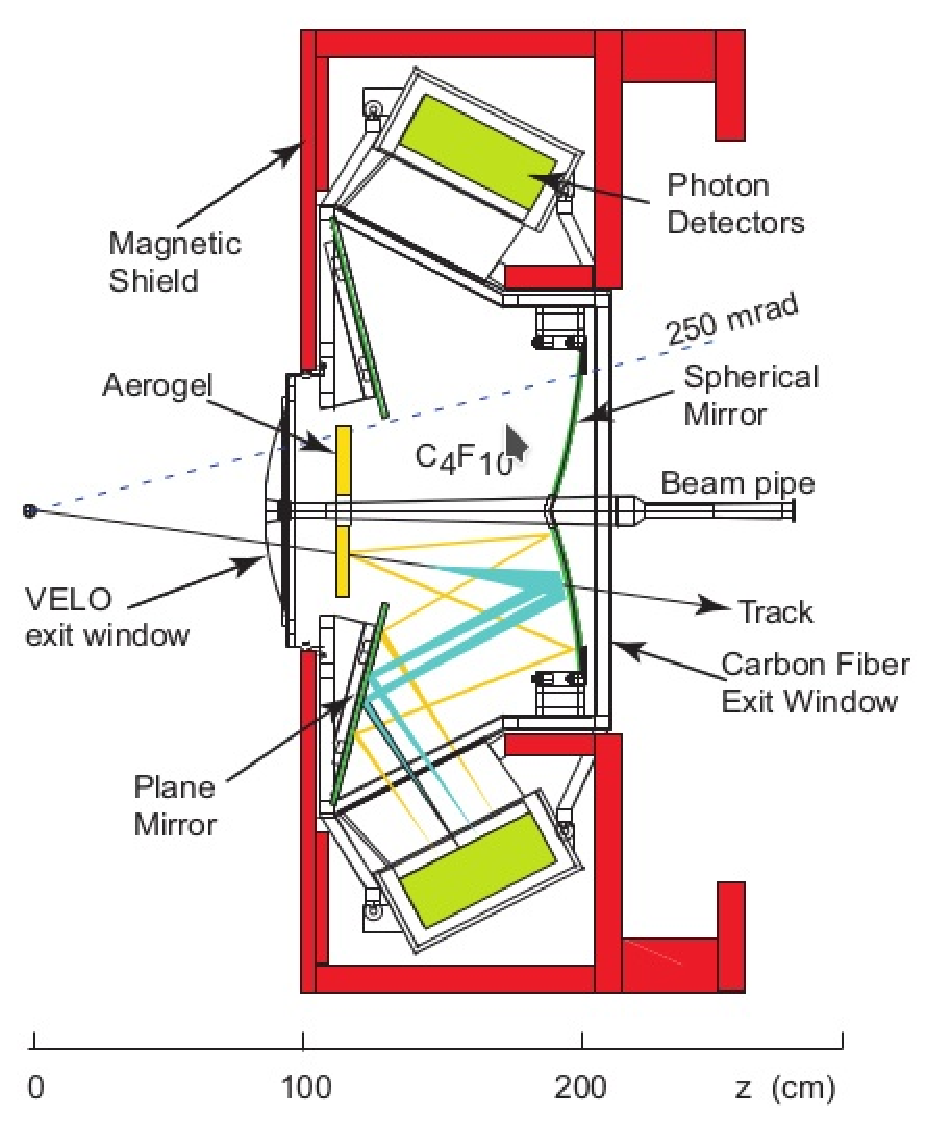
\includegraphics[width = 0.4\textwidth]{figs/detector/mechrich.eps}%
	\caption{Separation power for different species of particles in momentum-Cerenkov angle plane (left). Schematic diagram of RICH1 layout (right). Boths figures are taken from \cite{det_paper}.}
	\label{fig:richres}
\end{figure}

\section{RICH Reconstruction and Performance}
In order to establish species of particles for each track, the Cerenkov angle is combined with the track momentum measured by tracking. In practice, however, as \Gls{RICH} detectors operate in high track density environment, many Cerenkov rings will be overlapping and hence a complex pattern recognition algorithm is deployed \cite{Forty:1999sg}. 


For each event, the \Gls{RICH} computes full event likelihood that is consistent with assigning pion mass hypothesis for all tracks given the observed hit distribution read out by \Gls{HPD}. The algorithm then iterates through all other possible particle species, ($e, \mu, \pi, K,$ proton, deuteron), assigning new full event likelihood for a given track, having all other hypotheses fixed. The mass hypothesis with the highest full event likelihood is assigned to the track and this process is repeated for all the tracks in the event, until no improvement is found. 

Results of this algorithm provide likelihood variables, $DLL_{x}$, that quantify the strenght of the chosen species hypothesis against pion hypothesis,
\begin{equation}
	DLL_{x} = log(\mathcal{L})_{x} - log(\mathcal{L})_{\pi} \quad  x\in{e, \mu, K, proton, deuteron}.
\end{equation}

By calculating $DLL_{x_{1}} - DLL_{x_{2}}$, one can obtain discriminative strenght between any two species.

\subsection{RICH performance}
In order to measure the performance of the \Gls{PID} computed by RICH, populous calibration samples with very little background contamination are required. In order not to bias results, these samples have no \Gls{PID} constraints themselves and are reconstructed solely using kinematic information. For studies of pion/kaon efficiencies, $D^{*+} \to D^{0}(\kaon^{-}\pip)\pip$ backround-substracted samples are used, whereby the daughter tracks of $D^{0}$ become proxies for evaluation. The probability of correctly identifying kaon given certain constraint on $DLL_{K}$, identification efficiency (\Gls{ID}), and probability of mistakenly swapping pion identification, \Gls{misID} efficiency, are summarized in~\autoref{fig:richperf}. Identification probabilities of $\approx$ 85\% with misidentification rate of $\approx$ 3\% provide invaluable discriminating separation between kaon and pion.




\begin{figure}[!h]
	\centering
	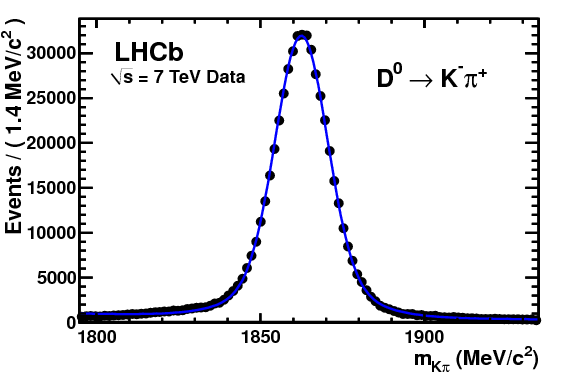
\includegraphics[width = 0.525\textwidth]{figs/detector/D0mass.png}%
	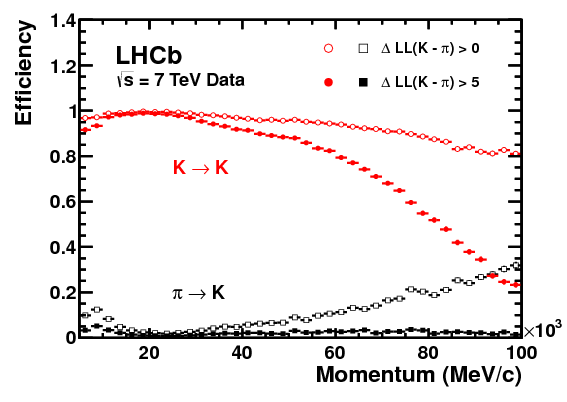
\includegraphics[width = 0.5\textwidth]{figs/detector/RICHperfdata.png}%
	\caption{Invariant mass distribution of $D^{0}$ data sample (in black) overlayed with fit to both background and signal (in blue) (left). An example of kaon \Gls{ID} (red) and \Gls{misID} (black) efficiency as a funtion of momentum under two PID hypotheses, $DLL_{K} > 0$ (empty)  and $DLL_{K} > 5$ (filled) (right). Boths figures are taken from \cite{LHCb-DP-2012-003}.}
	\label{fig:richperf}
\end{figure}

In search for $B^{0}$ and $B^{0}_{s}$ decaying to $h^{+}h^{-}$, where $h\in K, \pi$, $\pi^{+} \pi^{-}$ invariant mass spectra with and without PID $DLL_{x}$ requirements can be seen in~\autoref{fig:richnice}. These plots clearly demonstrate increase in sensitivity searching for $B^{0} \rightarrow \pi^{+} \pi^{-}$ signal amongst other components. 

\begin{figure}[!h]
	\centering
	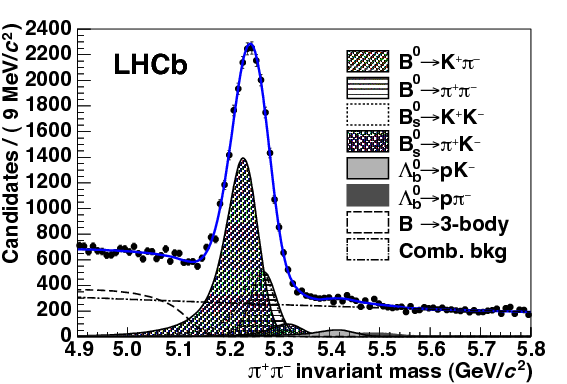
\includegraphics[width = 0.5\textwidth]{figs/detector/b2hhnopid.png}%
	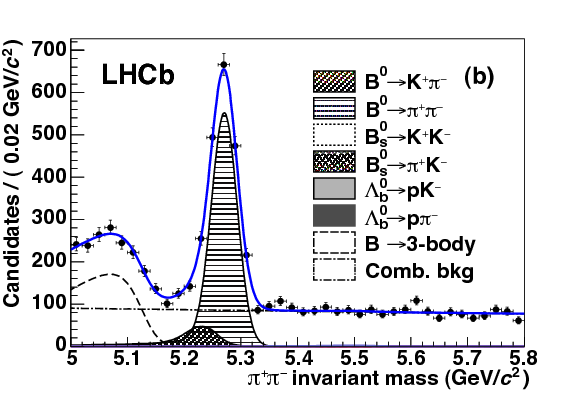
\includegraphics[width = 0.5\textwidth]{figs/detector/b2hhpid.png}%
	\caption{ $\pi^{+} \pi^{-}$ invariant mass distributions obtained using kinematic constraints only (left) and also using PID constraints (right) in order to isolate $B^{0} \rightarrow \pi^{+} \pi^{-}$ peak. This figure is taken from \cite{LHCb-PAPER-2012-002}. }  
	\label{fig:richnice}
\end{figure}


\section{Calorimetry}
As many other particle physics detectors, \Gls{LHCb} is equipped with series od subdetectors providing separation and \Gls{PID} tool for electrons, pions and photons. This separation is achieved because different particles interact at different distances, producing differently shaped showers of light. This part of detector is not only integral to the way \Gls{LHCb} trigger system works but it also provides precise measurement of energies of these objects.
All the subcomponents discussed here operate on the same principle. The light from the scintillating material is guided to photomultiplier tubes by wawelenght shifting fibres.

Electrons, pions and photons firstly encounter two planes of scintillating tiles: Scintillating Pad Detector (\Gls{SPD}), Preshower Detector (\Gls{PRS}) intersected by a wall of lead. The \Gls{SPD} senses the passage of charged particles whereas neutral particles will not be affected, distinguishing electrons from photons. The wall of lead initiates the electromagnetic shower, where photons are converted into electron-positron pairs, depositing sizable energy in the \Gls{PRS} allowing electron/pion separation. 

The following Elecromagnetic Calorimeter (\Gls{ECAL}) is based on sampling shashlik-type technology, where scintillating tiles are alternated by lead plates measuring the energy deposit of electromagnetic showers. As the best energy resolution requires full energy deposit of energetic photons along the \Gls{ECAL}, the thickness is eqvivalent to 25 radiation lengths. The resulting resolution of \Gls{ECAL} is $\frac{\sigma_{E}}{E} = \frac{10\%}{\sqrt{E}} \oplus 1\%$, where $E$ is in \gev.

On the other hand, \Gls{HCAL} sandwiches iron instead of lead as the absorber with thickness of 5.6 interaction lenght only, achieving resolution of $\frac{\sigma_{E}}{E} = \frac{70\%}{\sqrt{E}} \oplus 10\%$ in beam tests. This poorer resolution however fullfils the requirements necessary for the main purpose of this detector, hadron trigger. Away from beampipe the granularity of cells is coarser to mirror the track occupancy as seen in~\autoref{fig:CaloGran}. 

\begin{figure}[!h]
	\centering
	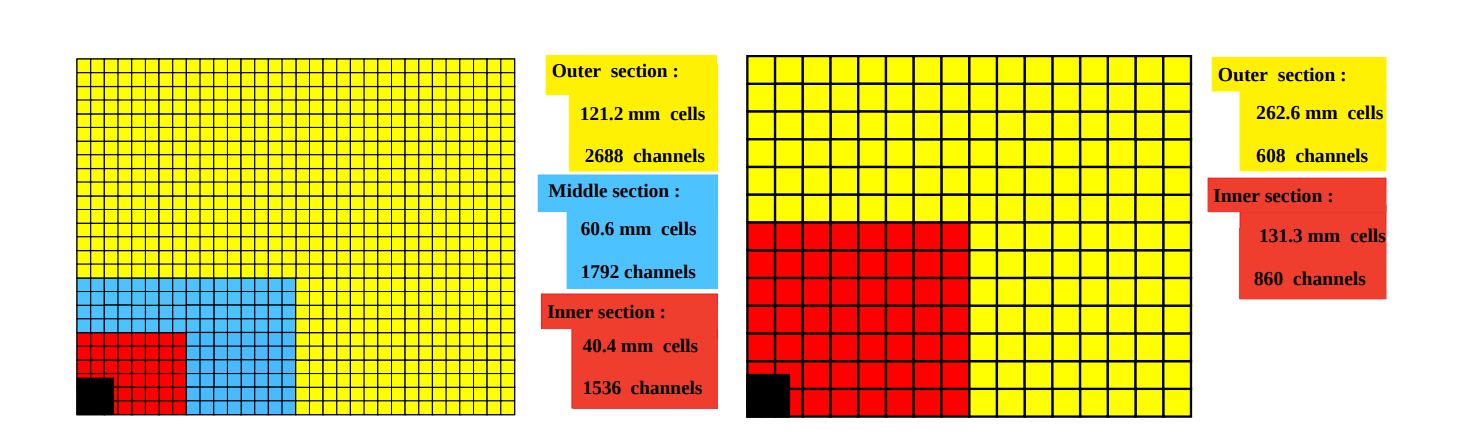
\includegraphics[width = 1.0\textwidth]{figs/detector/CaloGran.png}%
	%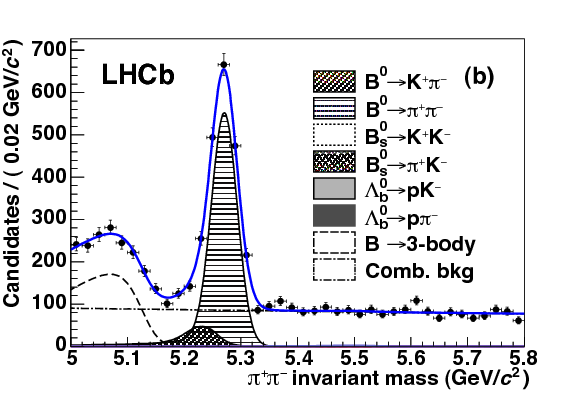
\includegraphics[width = 0.5\textwidth]{figs/detector/b2hhpid.png}%
	\caption{Granularity of \Gls{ECAL} (left) and \Gls{HCAL} (right) detectors. The figure was taken from \cite{det_paper}. }  
	\label{fig:CaloGran}
\end{figure}




\section{Muon Stations}
Muons are considered to be of fundamental importance to many flagship analyses by \Gls{LHCb}, such as the search for the rare $\B^{0}_{s} \rightarrow \mu^{+} \mu^{-}$ decay . Analysis of \Bmumumu ofcourse relies heavily on good performance of this part of detector. Muon stations are positioned at the end of the detector, taking advantage of the low probability of interaction of muon previously in the detector.

\Gls{LHCb}'s five rectangular muon stations \Gls{muonstation} are positioned before and after calorimetry system, with first station M1 upstream of the \Gls{SPD}, and four stations (M2-M5) downstream of \Gls{HCAL} as shown in~\autoref{fig:MuonGran}. The M1 station consists of 12 sets of three gas electron 
multiplier foils (triple-GEMs) in the region closest to the beam pipe, resisting the highest dose of radiation due to the highest particle flux. Its main use lies in improving the $p_{T}$ resolution by $\approx$ 10\%. M2-M5 station each consist of 276 multi-wire proportional chambers (\Gls{MWPCs}) filled with  $\rm{Ar-CO2-CF4}$ gas mixture. They are interlayed with 0.8\m iron walls, to provide stopping target to all particles, other than muons with momentum higher than $6$ GeV/c. In order to ease the accesibility, like in \Gls{VELO}, all the stations are split into two independent mechanical sides, also known A and C side.

Each station is then further segmented into four increasingly larger regions away from the beam, R1 to R4.
 All the regions were constructed to cover the same acceptance, keeping the track occupancy constant accross the station. The granularity of the readout is higher in the horizontal plane to take advantage of magnet's horizontal bending plane.




\begin{figure}[!h]
	\centering
	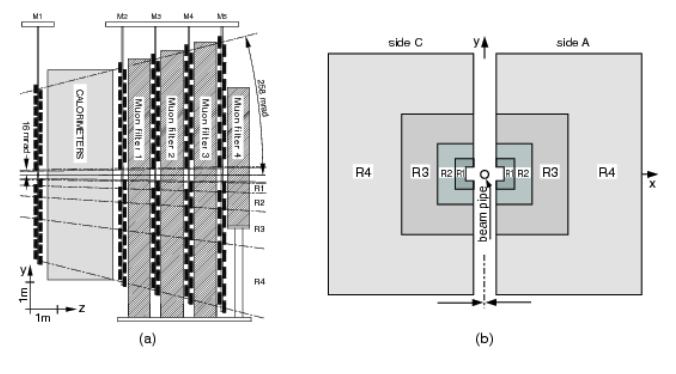
\includegraphics[width = 1.0\textwidth]{figs/detector/MuonGran.png}%
	%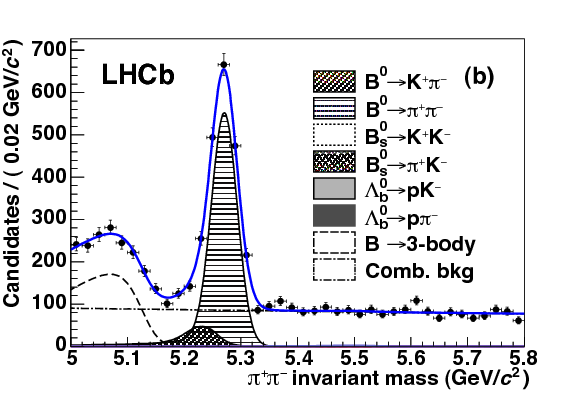
\includegraphics[width = 0.5\textwidth]{figs/detector/b2hhpid.png}%
	\caption{(a) Layout of the muon detector x-z plane and (b) x-y plane. This figure is taken from \cite{LHCb-DP-2012-002}. }  
	\label{fig:MuonGran}
\end{figure}

Both GEM and \Gls{MWPCs} operate on a same principle. In each station, position in the $x-y$ plane is determined by ionizing electrons that come from muons passing through the detector, which are then attracted either to the closest anode mesh or wire mesh. The trigger is fired if the corresponding rectangular region in each station enregistered positive binary decision. This means the efficiency of each station must be $\geq$99\% to give overall 95\% trigger efficiency. Geometrical layout covers $\approx$ 20\% muons originating in semileptonic $b$ decays.


\subsection{Muon Identification}
Apart from triggering events with high enough $p_{T}$ muons, muon stations provide necessary PID information for muon analyses. Offline variables mostly used for muon ID by analysts are
\begin{itemize}
	\item{\textbf{IsMuon}: Boolean decision of muon candidates with momentum-dependent categorisation. Long tracks with $p>3$\gev/c are extrapolated to muon stations yielding $x-y$ coordinates in $M2-M5$, considering only tracks within acceptance. For each station, search for the hit information within elliptical area defined by momentum, field of interest (\Gls{FOI}), is perfomed. The hit requirements are summarized in~\autoref{tab:ismuontab}.}
	\item{\textbf{muDLL}: Difference in log likelihoods computed using muon and non-muon hypothesis. These hypotheses are based on the proximity/distance $D^{2}$ of the track extrapolation into the muon stations and corresponding closest sensed hits in those stations. Muon-like particle will tend to have sharper distribution in $D^{2}$ as compared to other species. Protons were chosen for the calibration purposes giving broader distribution originating from punch-through protons, protons having concident hit position to true muon, and random hits.}
	\item{\textbf{DLLmu}}:  For each track global likelihood is produced, by combination of muon and non-muon likelihood from \textbf{muDLL}, with the \Gls{RICH} different mass hypothesis likelihoods, and calorimetry likelihood exploiting the energy deposits information. Like in \Gls{RICH} likelihoods, the default hypothesis corresponds to separation bewtween muon and pion hypothesis.    

\end{itemize}


\begin{table}[!h]
	\centering
	\hspace*{-0.8cm}
	\begin{tabular}{c c}
		\hline
		Particle Momentum $p$  & Hits in Muon Stations \\ \hline
		3 \gev/c <$p$<6 \gev/c & M1 $\&$ M2\\
		6 \gev/c <$p$<10 \gev/c & M1 $\&$ M2 $\&$ (M3 $||$ M4) \\
		10 \gev/c <$p$ & M1, M2, M3 and M4 \\ \\\hline      
	\end{tabular}
	\caption{Momentum-dependent definition \texttt{IsMuon} variable.}
	\label{tab:ismuontab}
\end{table}   

\subsection{Muon Performance}
As in hadron performance measurements, muon ID is determined using high statistics decay channel $J/\psi \rightarrow \mu^{+} \mu^{-}$ using tag-and-probe method. Mis-ID rates are computed using the same decay channels as previously. The summary of \texttt{IsMuon} \Gls{ID} and misID rates are presented in~\autoref{fig:MuonID}. Very high ID rate (above 90\%) for relatively low misID probability (below 10\%) performs the least well in low $p_{T}$ bins as here the muons end up outside of the acceptance. The misID rates for kaon and pions are significantly higher in low momenta region as the dominant process causing this are prompt muons from decay-in-flight.   

\begin{figure}[!h]
	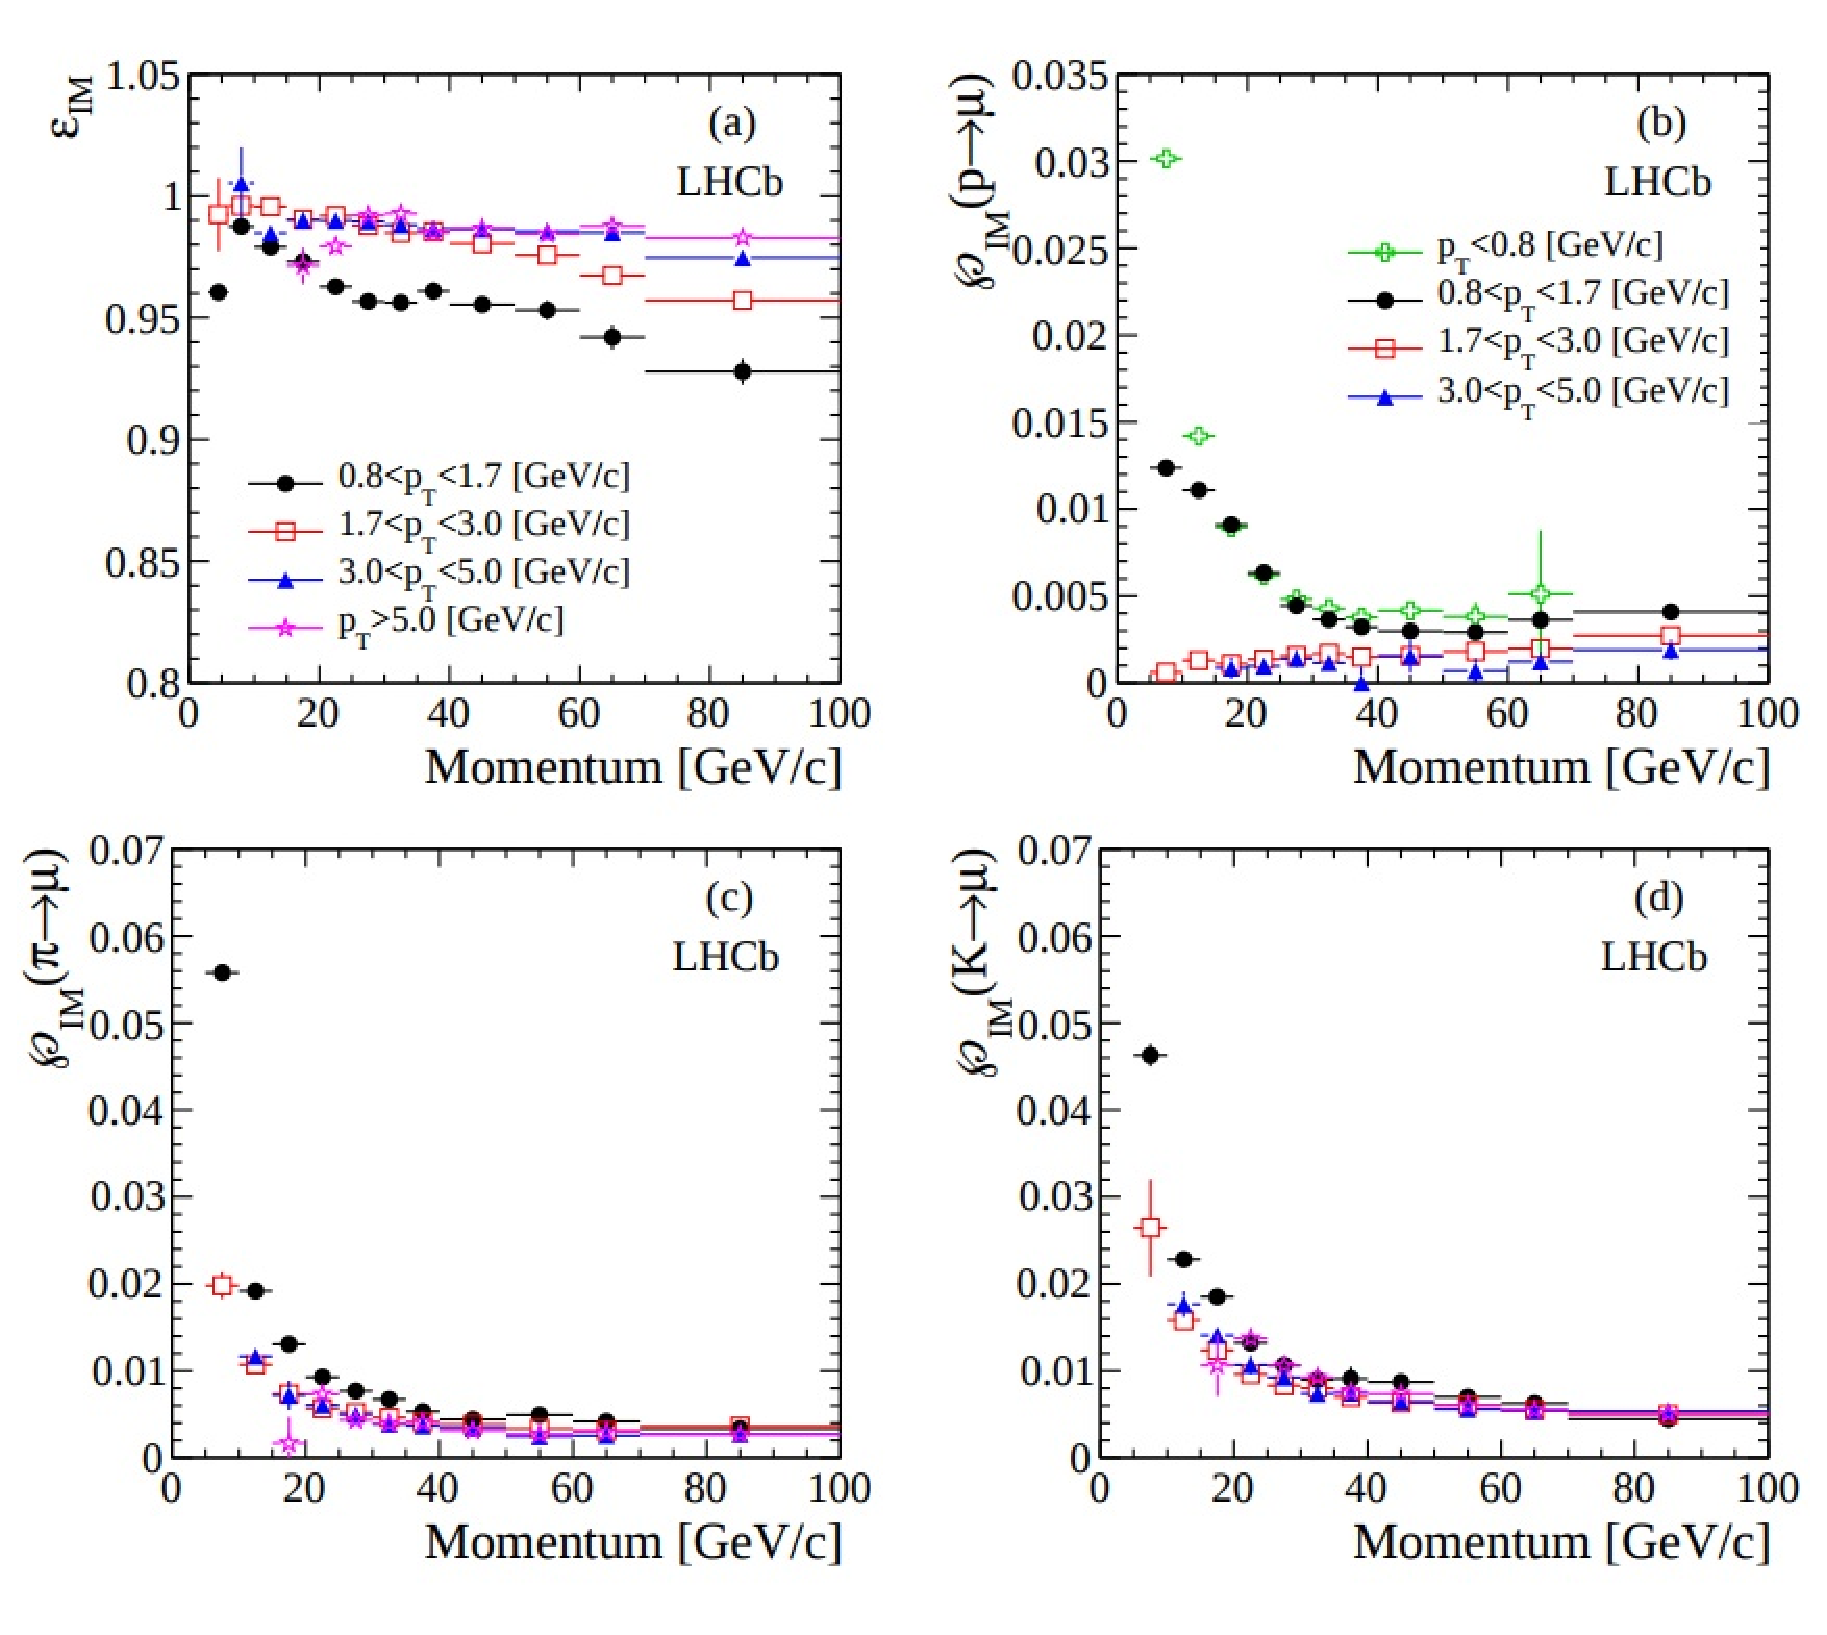
\includegraphics[width = 1.0\textwidth]{figs/detector/MuonPIDIsMuon.eps}%
	\caption{(a) Probability of correctly identifying muons as a function of momentum $p$ in the bins of $p_{T}$ for $J/\psi \rightarrow \mu^{+} \mu^{-}$ with \texttt{IsMuon} constraint. (c) Probability of incorrectly identifying pion (b) proton and (d) kaon as muon with \texttt{IsMuon}. This figure is taken from \cite{LHCb-DP-2013-001}. }  
	\label{fig:MuonID}
\end{figure}


\section{Trigger}
Nowadays, big-data physics experiments have to make decisions on what kind of data they want to keep. The choice of interesting events is performed by series of decisions, which is cumulatively known as trigger. \Gls{LHCb} trigger system was build around constraints posed by the run conditions, read-out capabilities and available disk space. In Run \Rn{1} and Run \Rn{2} LHCb has at its disposal the multistage trigger consisting of hardware-based level 0 trigger (\Gls{L0}) and software-based high level trigger (\Gls{HLT}).

\Gls{L0} reduces the rate of data from 40 \mhz to 1 \mhz by employing five trigger decisions, also known as lines. First three lines make desicion using calorimeter information about the transverse energy, $E_{T}$, whether it is photon, electron or hadron causing the shower energy deposit. Two other lines are reading out information from the muon system by looking for transverse momentum, $p_{T}$, of muon and dimuon (two muon tracks) objects. Efficiencies of L0 muon triggers are evaluated using $B^{+} \rightarrow (J/\psi \rightarrow \mu^{+} \mu^{-}) K^{+}$ decays. Hadron trigger efficiency in different decay channels can be seen in~\autoref{fig:L0Perf}. 


\begin{figure}[!h]
	\centering
	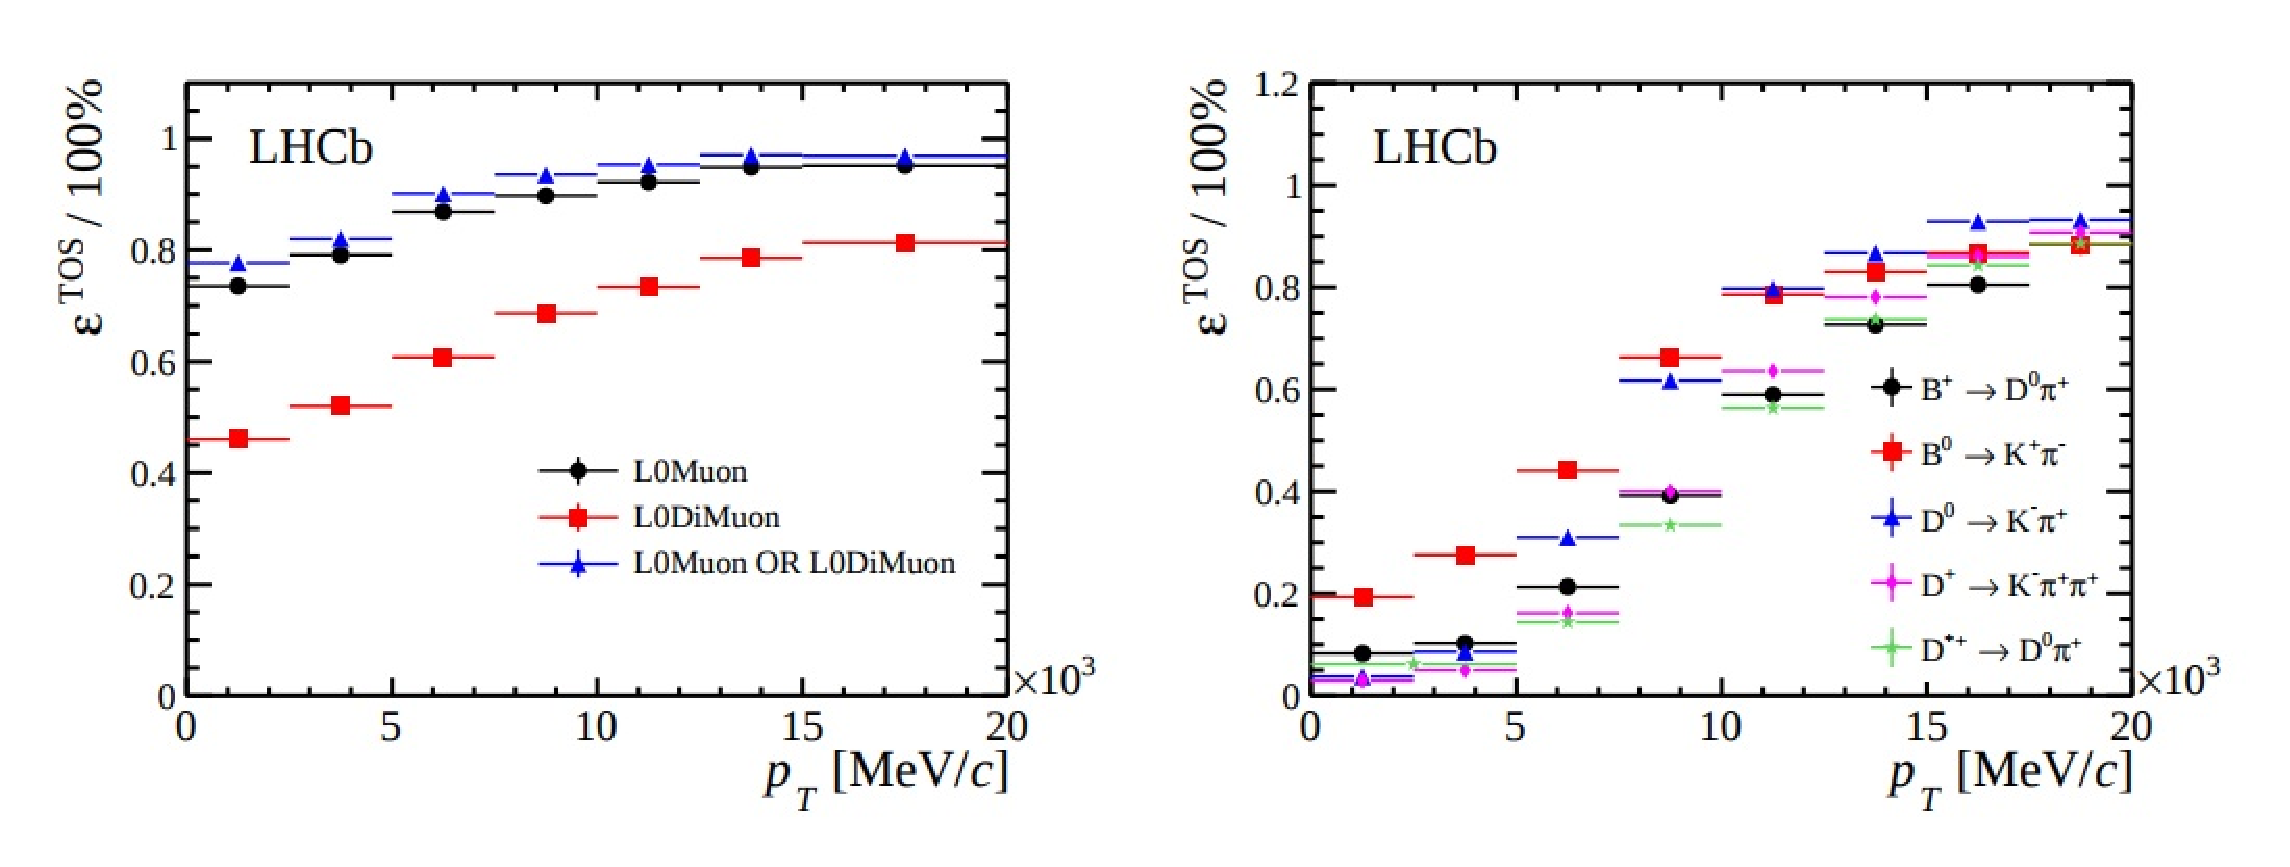
\includegraphics[width = 1.0\textwidth]{figs/detector/L0performance.eps}%
	%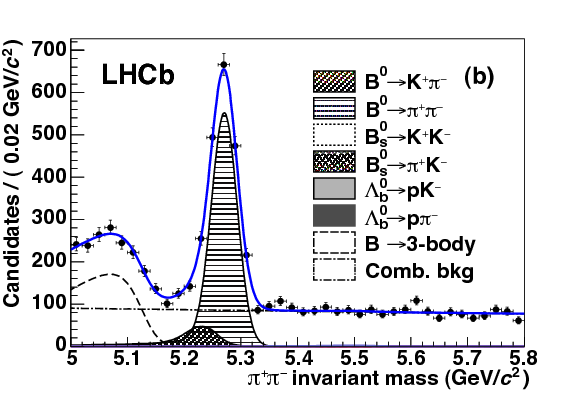
\includegraphics[width = 0.5\textwidth]{figs/detector/b2hhpid.png}%
	\caption{ \Gls{TOS} efficiency as a function of $p_{T}$ for muon-based decisions (left).         \Gls{TOS} efficiency for different decays using L0 hadron trigger lines. This figure is taken from \cite{LHCb-DP-2012-002}. }  
	\label{fig:L0Perf}
\end{figure}


Software-based \Gls{HLT} then further reduces the rate from 1 \mhz down to $40-80$ \khz which can be safely stored to disk. The first stage of the \Gls{HLT}, (\Gls{HLT1}), performs limited track reconstruction and hence makes decision based on the presence of charged tracks in the event. \Gls{HLT1} uses \Gls{VELO} hits to reconstructs \Gls{PV}s and \Gls{VELO} trakcs by using 3D pattern recognition. As \Gls{LHCb}'s primary mission is to study decays of hadrons containing $b$ and $c$ quark, \Gls{HLT1} will make decision based on the track segments being displaced (having high \Gls{IP}) with respect to the \Gls{PV}. For events selected by the $L0Muon$, an attempt is made to match the \Gls{VELO} tracks to hits observed in the vertical plane in the muon chambers due to magnet bending plane. By computing the track $\chi^2$, the potential muon track canditates are selected. Finally, the \Gls{VELO} tracks and muon tracks are extrapolated into the \Gls{OT} or \Gls{IT} trackers, allowing for so called \textit{forward tracking}, whereby $p$ and $p_{T}$ requirements are imposed to reduce processing time. Each track is then fitted with fast Kalman filter providing the $\chi^2$ of the fit. The corresponding performance of \Gls{HLT1} trigger lines are shown in~\autoref{fig:Hlt1Perf}.


\begin{figure}[!h]
	\centering
	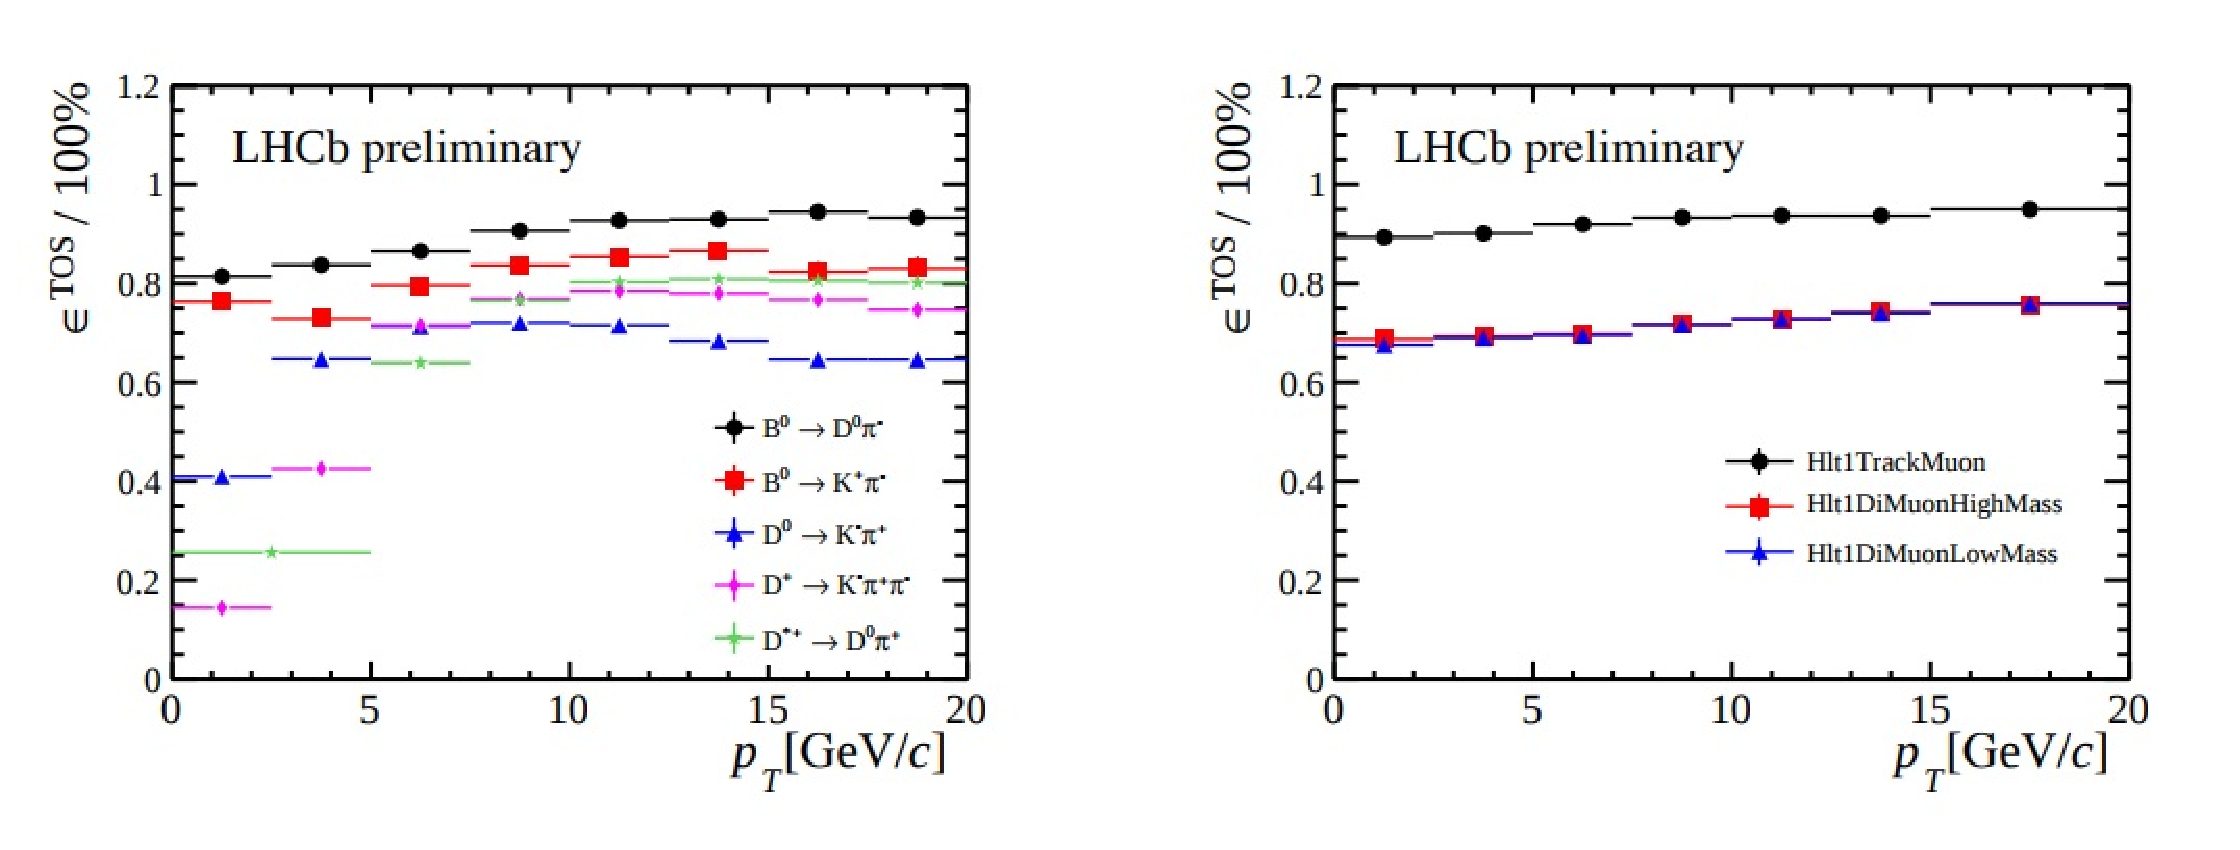
\includegraphics[width = 1.0\textwidth]{figs/detector/HLT1performance.eps}%
	%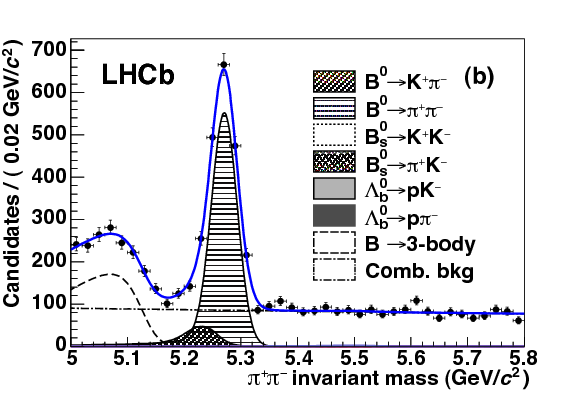
\includegraphics[width = 0.5\textwidth]{figs/detector/b2hhpid.png}%
	\caption{ \Gls{HLT1} efficiencies of the corresponding triggers using the same proxy as in~\autoref{fig:L0Perf}.  This figure is taken from \cite{Albrecht:2013fba}. }  
	\label{fig:Hlt1Perf}
\end{figure}

The second stage $\Gls{HLT2}$ reduces the rate to 5 \khz that can be safely written to disk. $\Gls{HLT2}$ consists of a series of decisions based on a full reconstruction of either groups of decays or specific decay modes. \textit{Topological triggers} exploit the vertex and track information (topology) of $b$-hadron decays. By employing multivariate techniques 2,3 or 4-body decays away from $PV$ are reconstructed. To account for decays where final state particle is not fully reconstructed, corrected mass serves as an input variable in the the \Gls{BDT}. Dedicted lines are also written to reconstruct muon and dimuon channels allowing for both prompt $J/\psi$ and $B\rightarrow J/\psi X$ studies. Finally \textit{Exclusive triggers} concentrating on selecting events with $c\bar{c}$ do selection very similar to the offline selection but without \Gls{PID} cuts and with \textit{prescales}, only allowed in a certain fraction of events, is applied.


In the end, selected events have their trigger decisions categorized by different type.  An event where signal candidate caused the trigger to fire is known to be Trigger on Signal (\Gls{TOS}). An event where it is non-signal like particle causing the trigger decision to occur, Trigger Independent of Signal (\Gls{TIS}) is used. Finally, if only by combination of signal particle together with other particle's properties in the event produce affirmative decision, then these events are categorized as \Gls{TIS} $\&$ \Gls{TOS} = \Gls{TISTOS}.

Between the Run \Rn{1} and Run \Rn{2} period there has been a change in how the software trigger operates, which can be seen in~\autoref{fig:TriggerChange}. As more timing budget was introduced for both \Gls{HLT1} and \Gls{HLT2}, \Gls{LHCb} took advatage in upgrading the trigger system. By introducing update of calibration and alignment constants of the relevant subdetectors before the data is sent to permanent disk, \textit{online reconstruction}, defined as being produced at trigger farm, is the same as the \textit{offline reconstruction}, defined as reconstruction made when data reached the permanent disk. Hence, there is enhancement of available information, such as the \Gls{PID} in the \Gls{HLT}, which can be then used at the trigger level. 
(Mention Turbo?).


\begin{figure}[!h]
	\centering
	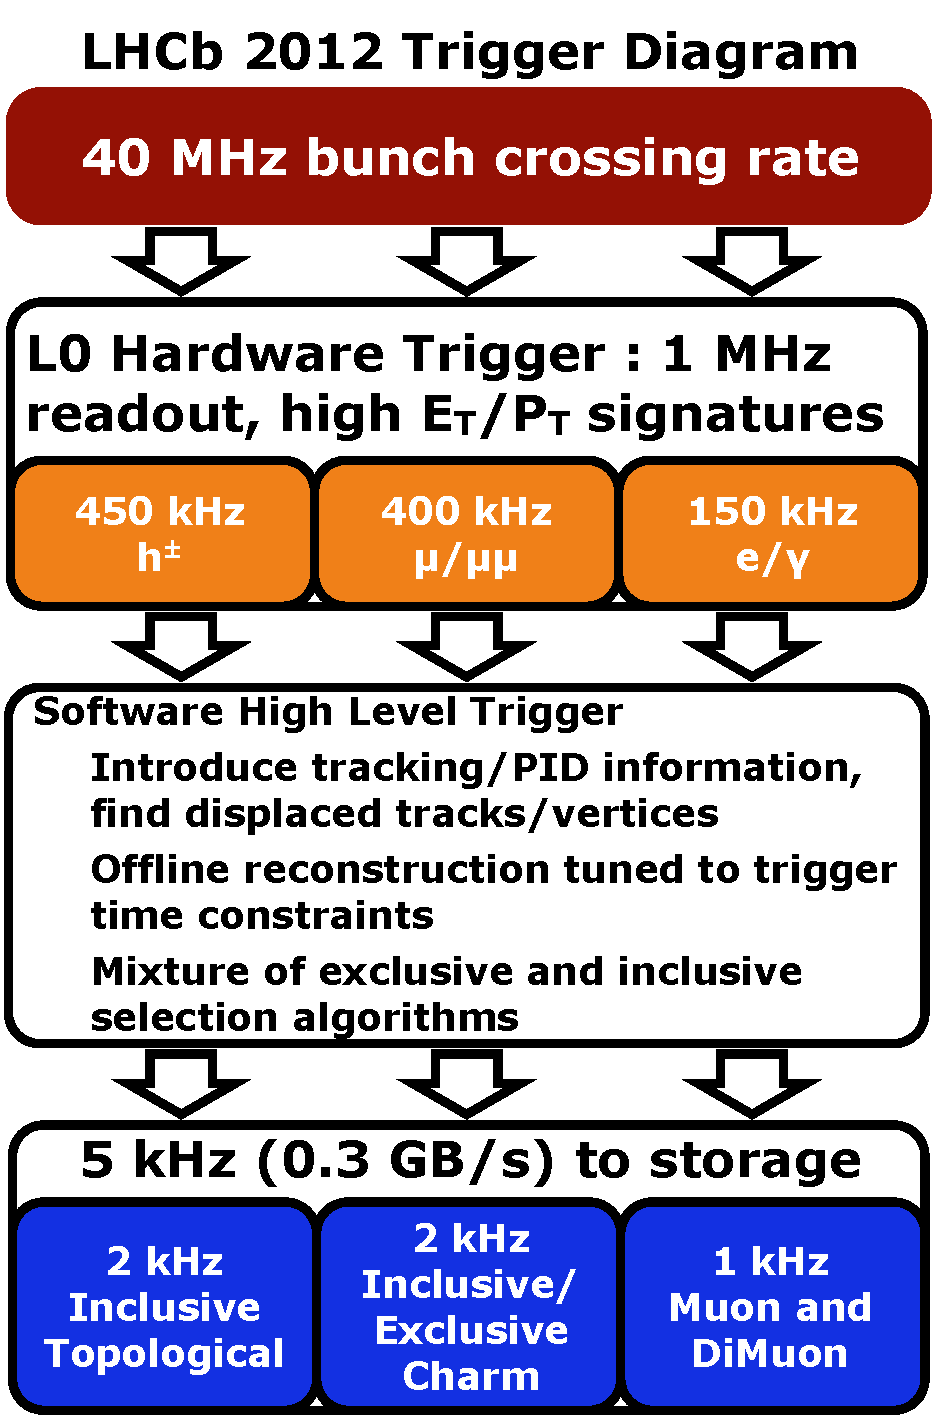
\includegraphics[width = 0.5\textwidth]{figs/detector/LHCb_Trigger_RunIAlg.pdf}%
	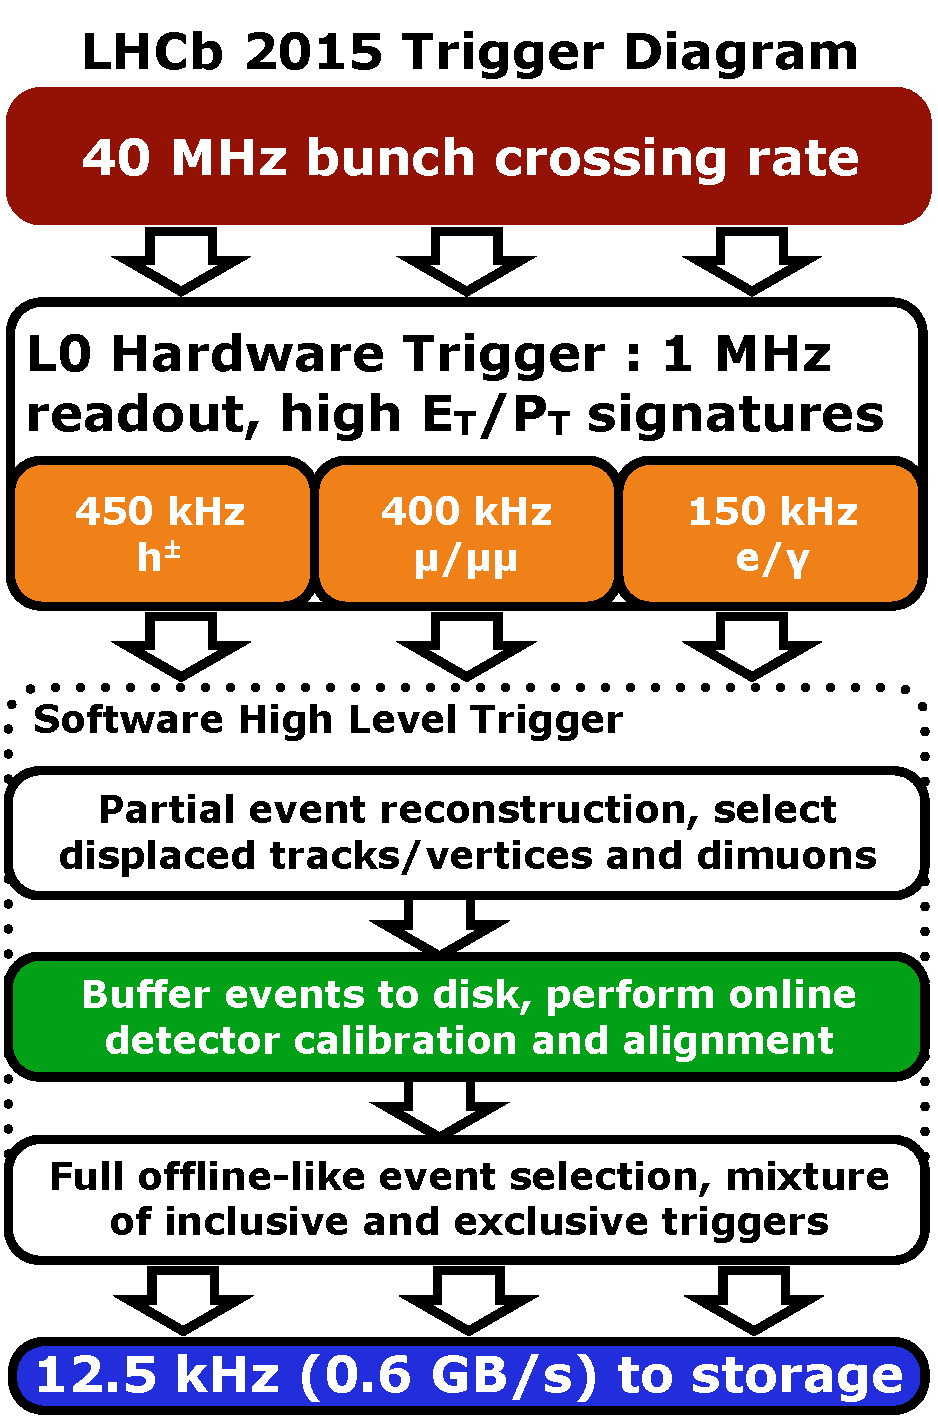
\includegraphics[width = 0.5\textwidth]{figs/detector/LHCb_Trigger_RunII.pdf}%
	%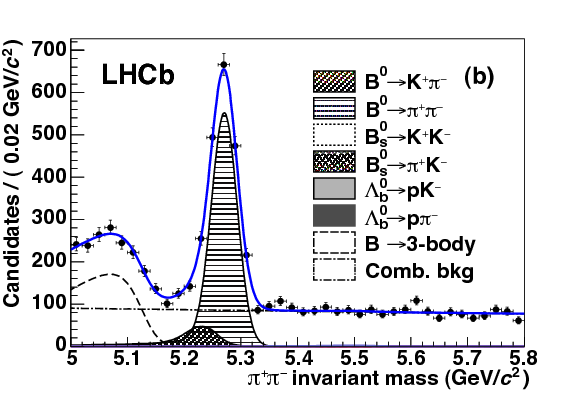
\includegraphics[width = 0.5\textwidth]{figs/detector/b2hhpid.png}%
	\caption{Trigger scheme differences between Run \Rn{1} and Run \Rn{2}. Figures obtained from \cite{triggerscheme}}  
	\label{fig:TriggerChange}
\end{figure}


\section{Simulation}
In order to optimise the event selections, extract efficiencies and model the backgrounds, a full Monte Carlo Simulation \Gls{MC} starting from simulation the $pp$ collision to detector readout of decay of interest is produced. 
The $pp$ collisions within \Gls{LHCb} configuration \cite{Belyaev:2011zza} are simulated with Pythia 6.4 \cite{pythia6} and Pythia 8.2 \cite{pythia8}. \Gls{LHCb} specific settings are mostly related to running conditions: luminosity, number of collisions per bunch crossing as well as contamination from other bunches, \textit{spill-over}. 

In the $pp$ collision, the $b$ and $c$ production mechanisms are simulated and then the following $b\bar{b}$ or $c\bar{c}$ pair is hadronized into hadrons of interest. In this thesis and the analysis presented, \Bp is the hadron of interest. Hadrons are then further decayed using EVTGEN \cite{Lange:2001uf} into the chosen decay products. In this stage, different physics models or inputs from theory can be configured. At the same time some initial CPU-friendly selection is established, usually requiring the hadrons to be contained within the forward detector's acceptance.
In order to account for the effects of \Gls{QED} radiative corrections, PHOTOS \cite{photos} algorithm can be used. All of this combined establishes \textit{generator-level simulation} of LHCb.


In the next phase, \textit{detector simulation}, the interactions of the all the particles with the detector, transport, as well as detector's response are simulated using the C++ GEANT4 toolkit \cite{Geant4},\cite{Agostinelli:2002hh}. \Gls{LHCb}'s interface to GEANT4 is detailed in \cite{Clemencic:2011zza}. 

\subsection{Differences in Simulation And Data}
Despite the complexity and best intention of the \Gls{LHCb} simulation, there are several shortcomings that require correction treatment.
The most afftected variables necessary for physics analyses that one needs to consider are \Gls{IP} resolution, track reconstruction efficiencies, \Gls{PID} variables and track occupancy.

The \Gls{IP} resolution shows better trend in the simulation then in the data due to the mismodelling of material description of \Gls{VELO} simulation. As shown in~\autoref{fig:IPRES} \Gls{IP} resolution does greatly differ depending the variation of material density of \Gls{VELO}. Around $\phi=\pm\pi/2$, where the two \Gls{VELO} parts overlap, the material difference causes the discrepancy. It can be corrected either by reweighting to data or by smearing the resolution wit Gaussian distribution.

\begin{figure}[!h]
	\centering
	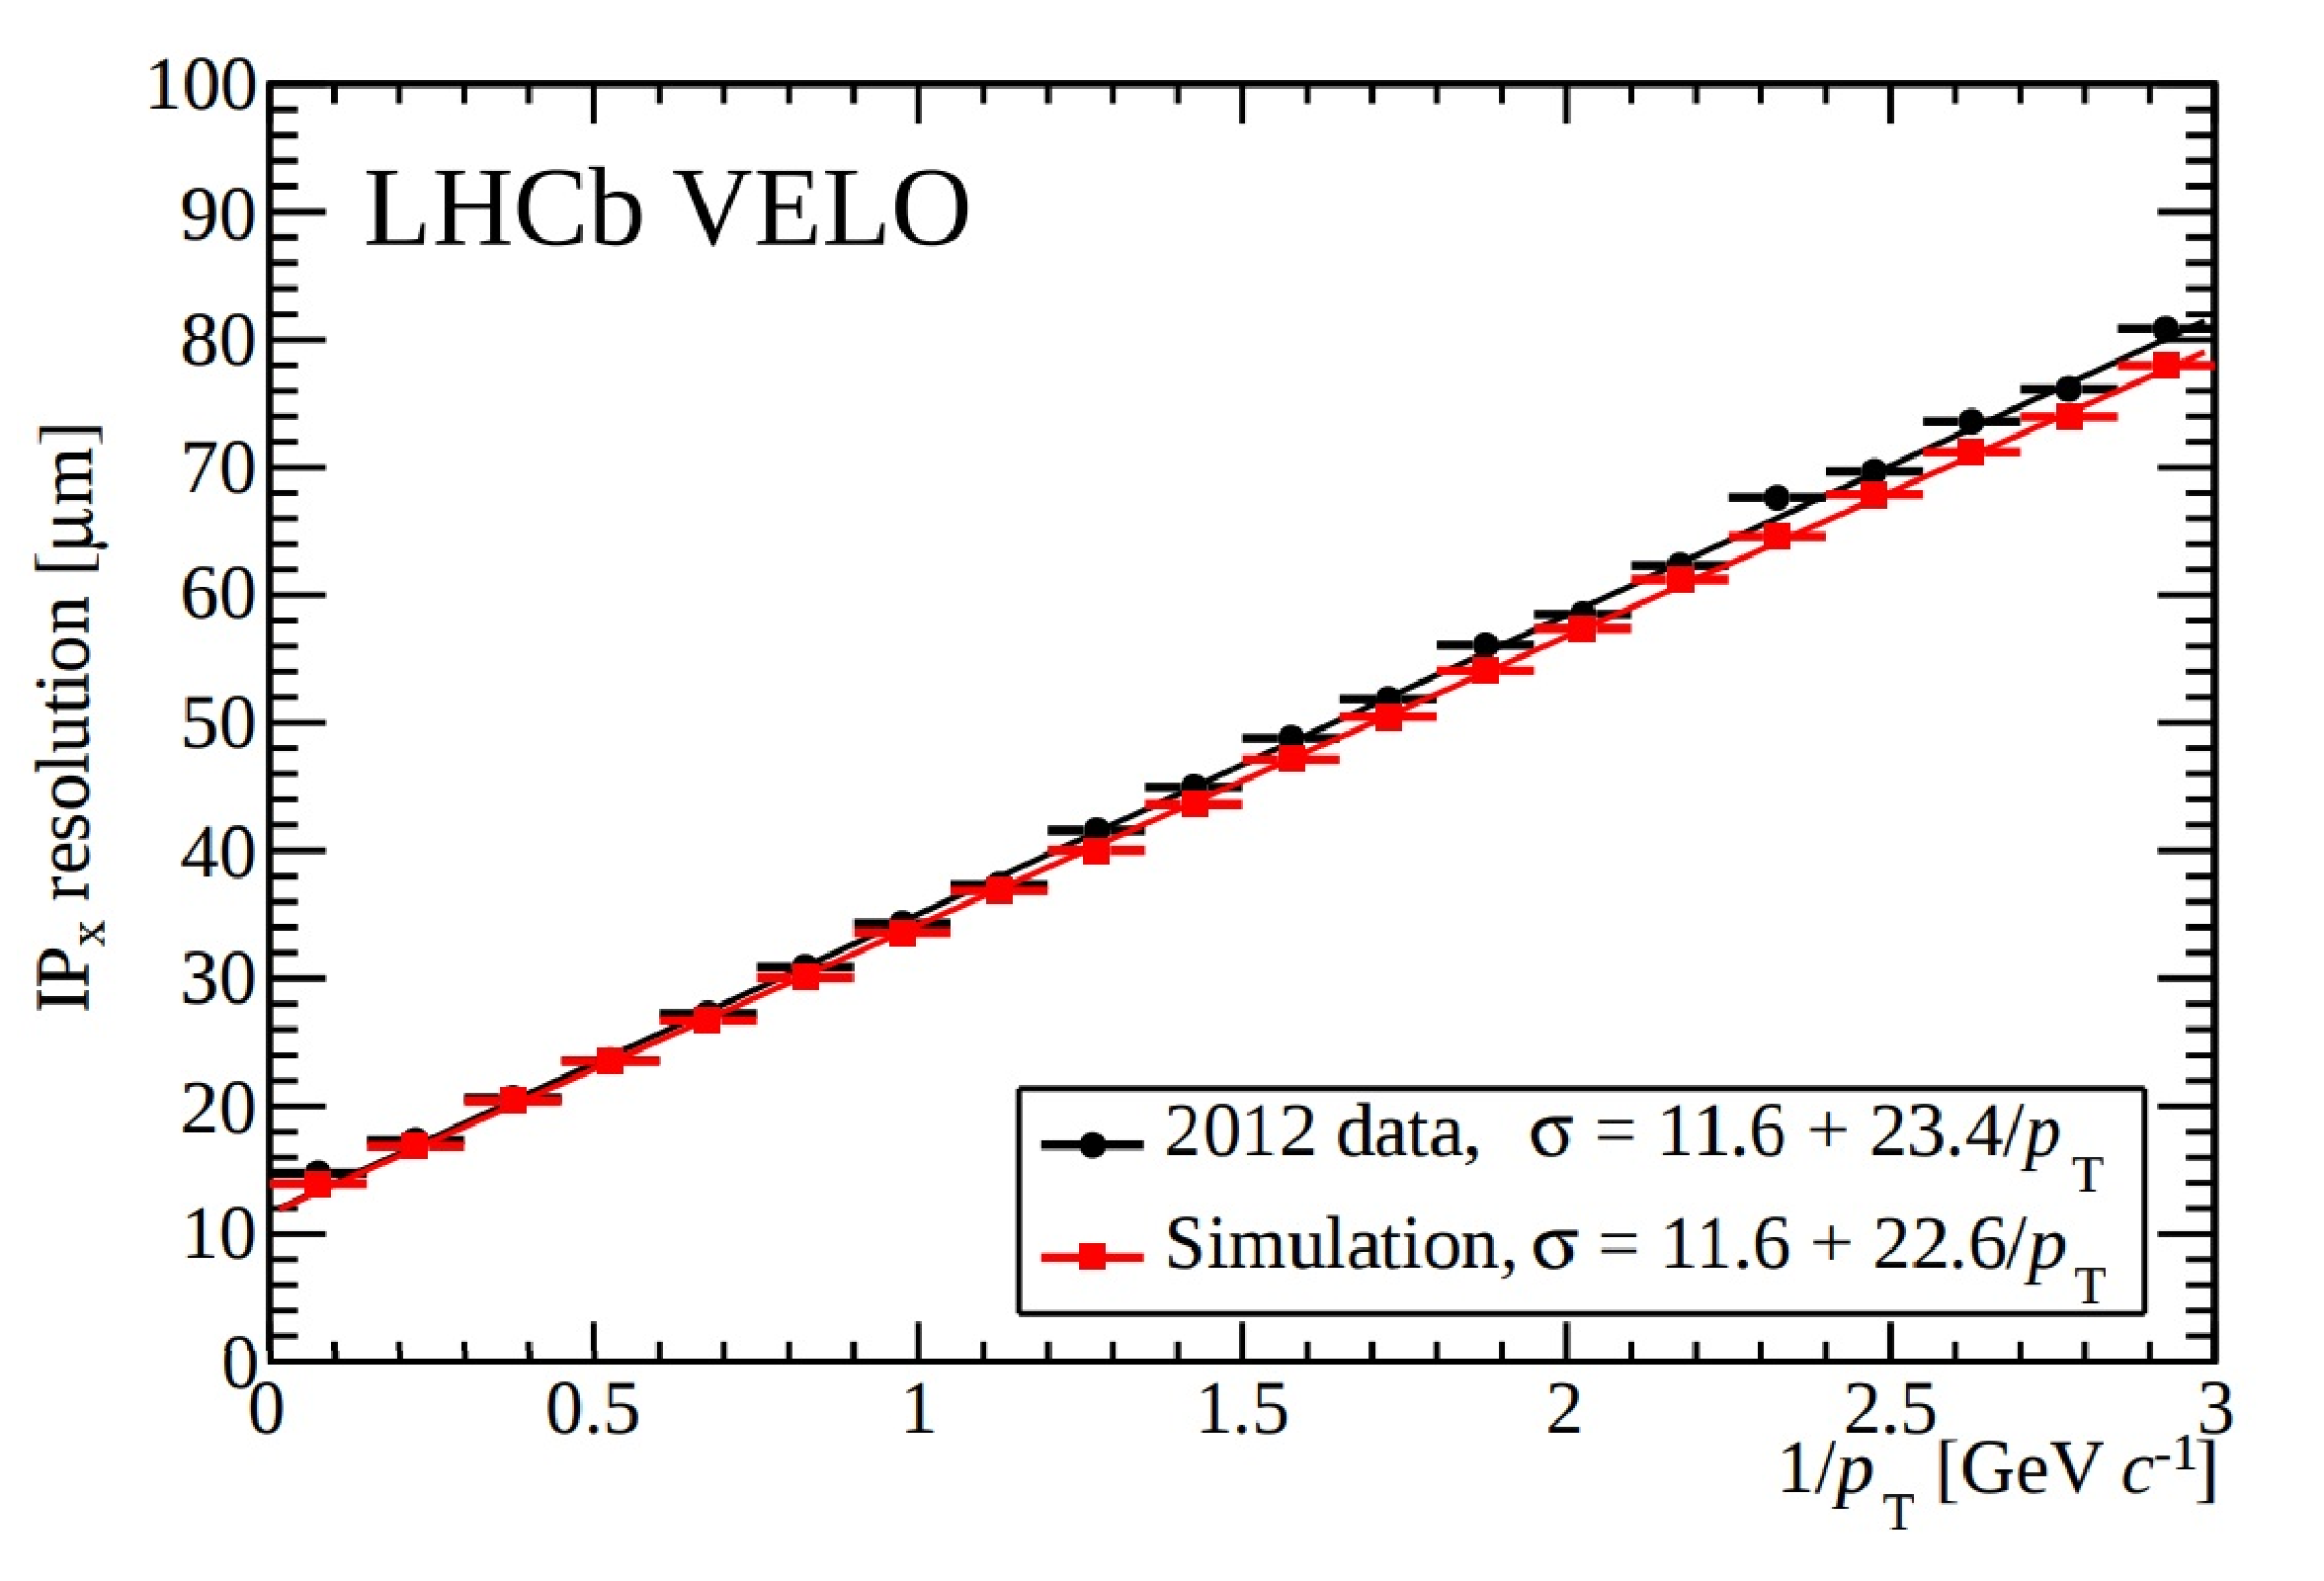
\includegraphics[width = 0.5\textwidth]{figs/detector/IPres.eps}%
	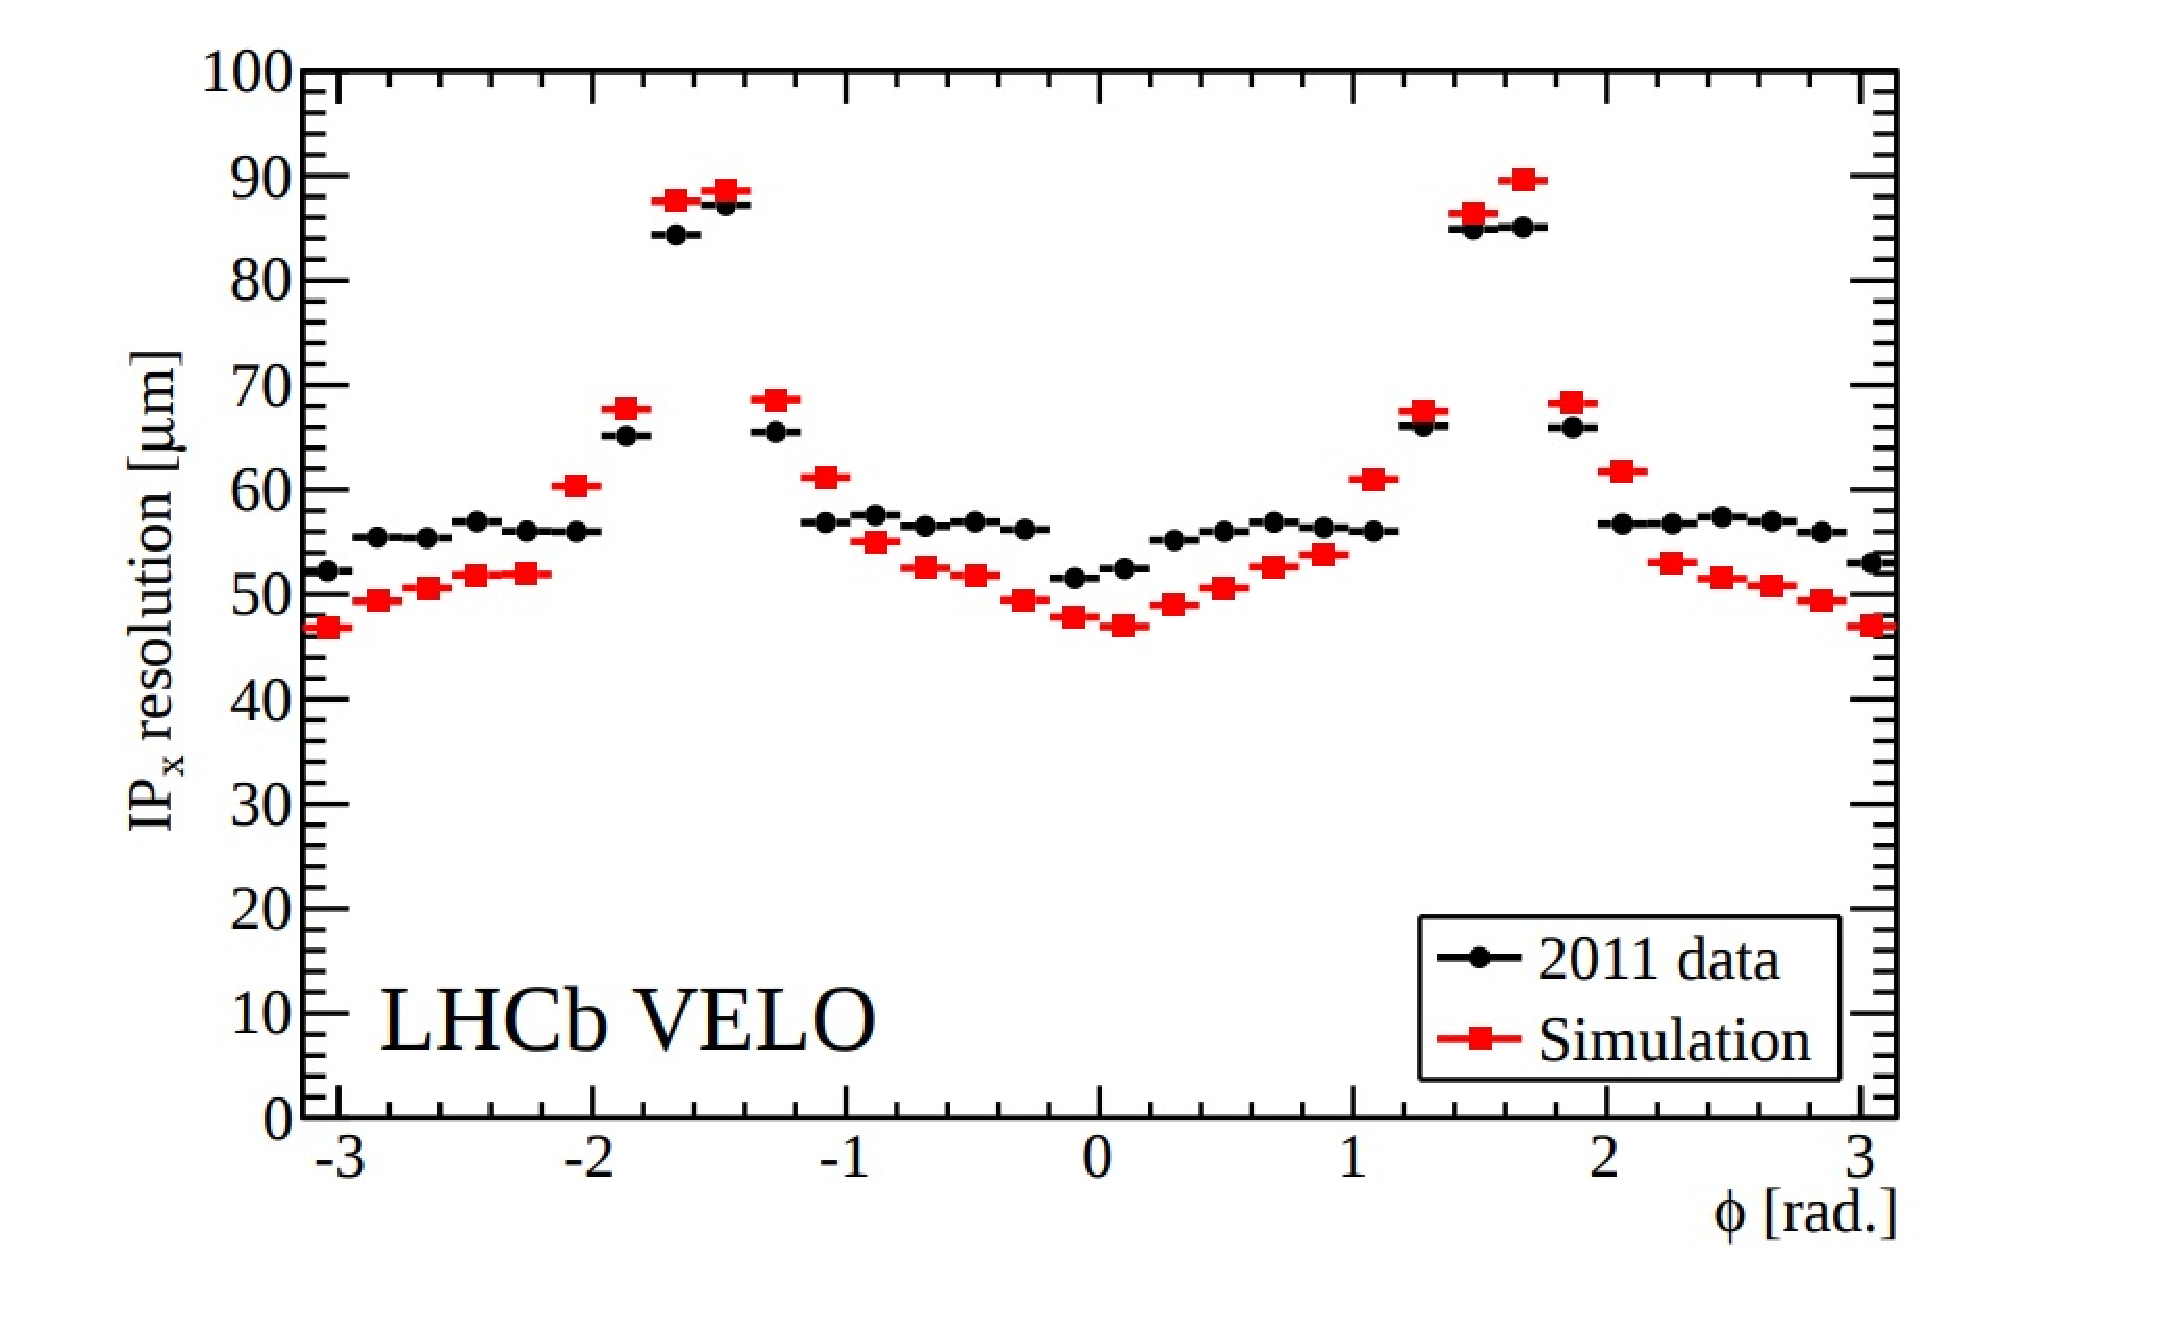
\includegraphics[width = 0.5\textwidth]{figs/detector/IPresAngle.eps}%
	\caption{\Gls{IP} resolution in x-direction comparing the data and simulation output for 2012 data-taking period (left). \Gls{IP} resolution in x-direction comparing the data and simulation output for 2011 data-taking period as a function of angle, $\phi$ (right). This figures are taken from \cite{LHCbVELOGroup:2014uea}. }  
	\label{fig:IPRES}
\end{figure}


Track reconstruction efficiency is also not reproduced very well in certain kinematical bins, again due to modelling of scattering interactions.

The most critical problem that needs to be addressed in the presented analysis are the inaccuracies of \Gls{PID} variables, which are mismodelled in the simulation. The origin of this problem arises as a consequence of much lower estimate of low momentum tracks in the detector making the photoelectron background underestimated. This results in better performace of separation power in simulation and is corrected using real data calibration.


